%% Copernicus Publications Manuscript Preparation Template for LaTeX Submissions

\documentclass[journal abbreviation, npg]{copernicus}

\begin{document}

\linenumbers

\title{Estimation of the total magnetization direction of approximately spherical bodies}

\author[1]{V.~C.~Oliveira Jr.}
\author[1]{D.~P.~Sales}
\author[1]{V.~C.~F. ~Barbosa}
\author[1, 2]{L.~Uieda}

\affil[1]{Observat\'orio Nacional, Rio de Janeiro, Brazil}
\affil[2]{Universidade do Estado do Rio de Janeiro, Rio de Janeiro, Brazil}

\runningtitle{Magnetization direction of spherical bodies}

\runningauthor{V.~C.~Oliveira Jr. et~al.}

\correspondence{V.~C.~Oliveira Jr. (vandscoelho@gmail.com)}

\received{5~August~2014}
\accepted{9~August~2014}
\published{}


\firstpage{1}

\maketitle  %% Please note that for the copernicus2.cls this command needs to be inserted after \abstract{TEXT}

\begin{abstract}
  We have developed a~fast total-field anomaly inversion to estimate
  the magnetization direction of multiple sources with approximately
  spherical shape and known centres. Our method is an overdetermined
  inverse problem that can be applied to interpret multiple sources 
  with different but homogeneous magnetization
  directions. It neither requires the prior computation of any
  transformation like reduction to the pole nor the use of regularly
  spaced data on a~horizontal grid. The method contains flexibility to
  be implemented as a~linear or non-linear inverse problem, which
  results, respectively, in a~least-squares or robust estimate of the
  components of the magnetization vector of the sources. Applications
  to synthetic data show the robustness of our method against
  interfering anomalies and errors in the location of the sources'
  centre. Besides, we show the feasibility of applying the upward
  continuation to interpret non-spherical sources. Applications to
  field data over the Goi\'{a}s Alkaline Province (GAP), Brazil, show
  the good performance of our method in estimating geological
  meaningful magnetization directions. The results obtained for
  a~region of the GAP, near from the alkaline complex of Diorama,
  suggest the presence of non-outcropping sources marked by strong
  remanent magnetization with inclination and declination close to
  $-70.35${\degree} and $-19.81${\degree}, respectively. This
  estimated magnetization direction leads to predominantly positive
  reduced-to-the-pole anomalies, even for other region of the GAP, in
  the alkaline complex of Montes Claros de Goi\'{a}s. These results show 
  that the non-outcropping sources near from the alkaline complex of 
  Diorama have almost the same magnetization direction of that
  ones in the alkaline complex of Montes Claros de Goi\'{a}s, strongly 
  suggesting that these sources have been emplaced in the crust almost 
  within the same geological time interval.
\end{abstract}

\introduction The magnetic method is one of the oldest geophysical techniques
and plays an important role in mineral and petroleum exploration. This method
underwent a~great progress after the advent of magnetometers properly
developed for airborne surveys. Nowadays, the combination of modern satellite
positioning systems and improvements in instrumentation and platform
compensation makes the aeromagnetic survey one of the most important 
data acquisition techniques due to the ability to cover large areas in a 
relative short period of time \citep{blakely1996,nabighian-etal2005}. 
The main applications
of the magnetic method are (i) estimating the average depth of the basement
relief, (ii) mapping geological faults and abrupt lithological contacts,
(iii) defining the limits of mineral targets, (iv) determining the location
of geological bodies like salt domes in sediments and (v) identifying
geological oil and gas traps. From the physical point of view, all these
geological scenarios can be associated to a~magnetization distribution
produced by magnetized rocks in subsurface. These magnetized rocks are the
magnetic sources producing a~magnetic induction that can be measured on the
Earth's surface or near from it. This magnetic induction causes local
differences between the measured data and the magnetic induction predicted by
global models describing the geomagnetic field. By isolating these local
deviations, the interpreter can determine the magnetic induction produced by
the magnetic sources making up the exploration targets.

The total field is the most common magnetic data measured in a~survey. It is
defined as the Euclidean norm of the magnetic induction produced by all
surrounding magnetic sources. After removing the Euclidean norm of the
magnetic induction predicted by a~global model describing the geomagnetic
field and correcting the wide range of undesirable artefacts affecting the
data, the result is a~scalar quantity denominated total-field anomaly. By 
using the total-field
anomalies, the geophysicist can characterize the magnetic sources in
subsurface and then better defining exploration targets
\citep{telford-etal1990,blakely1996}. Several widely used techniques 
for interpreting total-field 
anomalies require the correct knowledge of the magnetization 
direction of the sources. Among these techniques we emphasize 
the reduction to pole \citep{baranov1957,baranov-naudy1964,silva1986}, 
the pseudogravity transformation \citep{baranov1957} and the amplitude 
of the analytic signal \citep{nabighian1972,nabighian1974, 
nabighian1984,li2006}. Besides, several widely used magnetic inversion 
methods for estimating the distribution of the magnetization-intensity 
contrasts in the subsurface also require the knowledge of the correct 
magnetization direction \citep{li-oldenburg1996, pilkington1997,
portniaguine-zhdanov1999, portniaguine-zhdanov2002, barbosa-silva2006}.
Several methods for determining the magnetization direction of
the sources have been developed due to its great importance in
interpreting total-field anomalies. Recently, \citet{clark2014} presented an 
outstanding and comprehensive review of methods that determine the remanent 
and total magnetizations of magnetic sources. Here, we present only that 
ones related to our work.

We divide the methods for retrieving the magnetization direction into two
groups. The first one comprises methods that do not impose strong constraints
on the shape of the sources. \citet{fedi-etal1994}, for example, accomplished
successive RTP's in the wavenumber domain by using different tentative
magnetization directions. Among this set of RTP anomalies, these authors
choose that one whose amplitude of the negative part is minimum. Since this
method uses a wavenumber approach, it requires that the total-field anomaly
be regularly spaced in a horizontal grid with constant height to achieve the
computational efficiency of the FFT. Besides, it is known that the RTP in the
wavenumber domain is unstable at low latitudes and cannot be applied for
interpreting total-field anomalies produced by magnetic sources having
different magnetization directions. \citet{medeiros-silva1995} used the
source moments up to second order derived from the multipole expansion of the
magnetic potential for estimating the magnetization direction and the spatial
orientation of a magnetic source. Although this method does not strongly
constraint the source's shape, it presumes that the magnetic source has three
orthogonal planes of symmetry intersecting each other at the centre of the
source. It is also presumed that the source is far from the observation
points. \citet{phillips2005} proposed a method based on the numerical
evaluation of the integrals developed by \citet{helbig1963} for estimating
the magnetization direction and the location of multiple magnetic sources
from their first-order magnetic moments. \citet{phillips2005} stresses 
that the method
is useful for rapid analysis of gridded magnetic data and works best for
isolated and compact sources and largely fails for horizontally elongated
sources. \citet{tontini-pedersen2008} extended this method for using the
magnetic moments up to second order to obtain additional information about
the horizontal and vertical positions of the centre of the magnetization
distribution. \citet{dannemiller-li2006} extended the method proposed by
\citet{roest-pilkington1993}, who tackled total-field anomalies produced by
generalized 2-D sources, to estimate the magnetization direction of 3-D
sources by using the correlation between the vertical gradient and the total
gradient of the RTP anomaly obtained through a set of trial directions. These
authors stressed that the method assumes that the total-field anomaly is
produced by a set of 3-D causative bodies with the same magnetization
direction and not by multiple sources with different magnetization
directions. A similar method was proposed by \citet{gerovska-etal2009} based
on the comparison between the RTP anomaly and the total magnitude anomaly.
\citet{lelievre-oldenburg2009} developed a very flexible method for
estimating the magnetization vector distribution in complex geological
scenarios. This method discretizes the subsurface of the Earth into a grid of
3-D prisms and estimates the three components (in Cartesian or spherical
coordinates) of the magnetization vector of each cell by imposing strong
constraints on the solution to deal with the nonuniqueness. Recently,
\citet{ellis-etal2012} presented a similar method to interpret magnetic data
in mineral exploration surveys.

The second group of methods to estimate the magnetization direction of
the sources assumes the knowledge of the shape of the source. The
methods belonging to this group have led to a few published
papers. \citet{bhattacharyya1966}, for example, proposed an iterative
method for determining the magnetization of a uniformly magnetized
rectangular prism. The performance of this method is highly dependent
on the correct position of the centre and on the determination of the
major and minor axes of the body. \citet{emilia-massey1974} developed
an iterative method for estimating the vertical magnetization
distribution of seamounts. This method approximates the seamounts by
vertically juxtaposed right prisms having polygonal horizontal cross
sections, which have the same magnetization direction and different
magnetization intensities. \citet{parker-etal1987} also developed
a method for estimating the magnetization direction of seamounts. This
method was formulated as an optimization problem, named seminorm
minimization, to allow estimating a magnetization distribution that is
as close as possible to the uniform distribution. However, in
practical applications, this constraint may yield a poor data
fit. Finally, \citet{kubota-uchiyama2005} discretized the seamount
volume as a grid of juxtaposed right rectangular prisms and estimated
the Cartesian components of the magnetization vector of each prism.

In this work, we present a computationally efficient method for inverting the
total-field anomaly produced by multiple sources with approximately spherical
shape to estimate their magnetization directions. We assume sources with
known centre, which can be provided by Euler deconvolution, for example. The
proposed method is part of the group of methods imposing assumptions about
the shape of the magnetic sources. This assumptions about the underlying 
sources is able to reduce the nonuniqueness of the problem to a point that 
regularization or constraints are not required. Our method can be applied 
for estimating the average magnetization direction of
multiple sources. It neither requires that all sources have the same 
magnetization direction nor the use of regularly spaced data on a horizontal
grid. Besides, our method also contains
flexibility to be implemented in two different numerical approaches. The
first one minimizes an L2-norm, resulting in a linear inverse problem to
obtain a least-squares estimate. The second approach comprises the iterative
minimization of an L1-norm, resulting in a non-linear inverse problem to
obtain a robust estimate. Applications to synthetic data show the robustness
of our method against interfering anomalies and errors in the location of the
sources' centre. Additionally, we show how the upward continuation can be
used to make possible the application of our method to interpret
non-spherical sources. Applications to field data over the Goi\'{a}s Alkaline
Province (GAP), Brazil, show the good performance of the proposed method in
estimating geological meaningful magnetization directions. The obtained
results over a region of the GAP, near from the alkaline complex of Diorama,
suggest the presence of non-outcropping sources with strong remanent
magnetization, corroborating previous works. The estimated inclinations and
declinations are close to $-70.35${\degree} and $-19.81${\degree},
respectively.

\section{Methodology}

\subsection{Parameterization and forward problem}

Let $\vec{\Delta T}^\mathrm{o}$ be the observed data vector, whose $i$th
element $\Delta T^\mathrm{o}_{i}$, $i = 1, \ldots, N$, is the total-field
anomaly measured at the position ($x_{i}$, $y_{i}$, $z_{i}$) (black dots in
Fig.~\ref{fig:geometric-aspects}). In this Cartesian coordinate system, $x$
points to the geographic north, $y$ points to east and $z$ points downward.
In general, the total-field anomaly is produced by a distribution of 
magnetization which is anomalous with respect to the mean induced magnetization
of the crust. Mathematically, $\Delta T^\mathrm{o}_{i}$ can be
written as
\begin{align}
 &
\Delta T^\mathrm{o}_{i} = \Vert \vec{T}_i \Vert - \Vert \vec{F}_i \Vert ,
\label{eq:tfanomaly-i}
\end{align}
where $\Vert \cdot\Vert$ indicates the Euclidean norm, $\vec{F}_i$ is the
geomagnetic field vector and $\vec{T}_i$ is the total-field vector, both at
($x_{i}$, $y_{i}$, $z_{i}$). The total-field vector can be represented by the
sum
\begin{align}
 &
\vec{T}_i = \vec{F}_i + \vec{B}_i ,
\label{eq:tfvector-i}
\end{align}
where $\vec{B}_i$ is the total magnetic induction vector produced by all
magnetic sources (magnetized anomalous susceptibility distribution) at the
position ($x_{i}$, $y_{i}$, $z_{i}$) \citep{blakely1996,langel-hinze1998}.

For local or regional scale magnetic studies, it is very common to consider
that (i) the geomagnetic field $\vec{F}_i$ (Eq.~\ref{eq:tfanomaly-i}) is
a constant vector $\vec{F}_{0}$ throughout the study area and (ii) that
$\Vert \vec{F}_{0} \Vert\,\gg\, \Vert \vec{B}_{i} \Vert$, $i = 1, \ldots, N$
\citep{telford-etal1990,blakely1996}. The second assumption is equivalent to
say that the total magnetic induction $\vec{B}_i$ (Eq.~\ref{eq:tfanomaly-i})
is a small perturbation of the geomagnetic field $\vec{F}_i$ throughout the
study area. These two assumptions make possible to approximate the Euclidean
norm of the total-field vector $\vec{T}_i$ (Eq.~\ref{eq:tfanomaly-i}) by
a first-order Taylor's expansion as follows
\begin{align}
\begin{aligned}
\Vert \vec{T}_{i} \Vert & \approx\, \Vert \vec{F}_{0} + \vec{B}_{i} \Vert \\
 &\approx\, \Vert \vec{F}_{0} \Vert + \hat{\vec{F}}^{\mathrm{T}}\vec{B}_{i} ,
\end{aligned}
\label{eq:total-field-app}
\end{align}
where the superscript $\mathrm{T}$ indicates transposition and
\begin{align}
 &
\hat{\vec{F}} = \frac{\vec{F}_{0}}{\Vert \vec{F}_{0} \Vert}
\label{eq:unit-vector}
\end{align}
is a unit vector (with the same direction of the geomagnetic field
$\vec{F}_i$) representing the gradient of the function $\Vert
\vec{T}_{i} \Vert$ with respect to the components of the vector
$\vec{T}_{i}$ \citep{blakely1996}. By introducing this first-order
Taylor's expansion into the total-field anomaly
(Eq.~\ref{eq:tfanomaly-i}), we obtain the well-known approximated
total-field anomaly given by
\begin{align}
 &
\Delta T_{i} \approx \hat{\vec{F}}^{\mathrm{T}}\vec{B}_{i} , \qquad i = 1, \ldots, N .
\label{eq:approx-tfanomaly-i}
\end{align}

Let's consider that the magnetic sources can be represented by a set
of $L$ uniformly magnetized spheres. In this case, the total magnetic
induction $\vec{B}_i$ is given by
\begin{align}
 &
\vec{B}_i = \sum_{j = 1}^{L} \vec{b}_{i}^{j} , \qquad i = 1, \ldots, N ,
\label{eq:total-induction-i}
\end{align}
being $\vec{b}^{j}_{i}$ the magnetic induction produced, at the position
($x_{i}$, $y_{i}$, $z_{i}$), by the $j$th sphere, $j = 1, \ldots, L$, with
radius $R_ {j}$ (dashed straight lines in Fig.~\ref{fig:geometric-aspects}),
centre at $(xc_{j}$, $yc_{j}$, $zc_{j}$) (grey dots in
Fig.~\ref{fig:geometric-aspects}) and magnetization vector $\vec{m}^{j}$
given by
\begin{align}
 &
\vec{m}^{j} =
\begin{bmatrix}
mx_{j} \\
my_{j} \\
mz_{j}
\end{bmatrix}_ {3 \times 1} .
\label{eq:mag-vector-j}
\end{align}
The magnetic induction $\vec{b}^{j}_{i}$ (Eq.~\ref{eq:total-induction-i}) can
be written as
\begin{align}
 &
\vec{b}^{j}_{i} = C_{m}  \mathbf{M}_{i}^{j}
                  \frac{4}{3} \pi R_{j}^{3}
                  \vec{m}^{j} ,
\label{eq:j-induction-i}
\end{align}
where $C_{m}$ is a constant given by $\mu_{0}/{4 \pi}=10^{-7}$ $H/m$,
$\mu_{0}$ is the vacuum permeability and $\mathbf{M}_{i}^{j}$ is the
matrix
\begin{align}
 &
\mathbf{M}^{j}_{i} =
\begin{bmatrix}
\left(\frac{\partial^{2}}{\partial x \partial x} \frac{1}{r_{j}} \right) &
\left(\frac{\partial^{2}}{\partial x \partial y} \frac{1}{r_{j}} \right) &
\left(\frac{\partial^{2}}{\partial x \partial z} \frac{1}{r_{j}} \right) \\[2mm]
\left(\frac{\partial^{2}}{\partial x \partial y} \frac{1}{r_{j}} \right) &
\left(\frac{\partial^{2}}{\partial y \partial y} \frac{1}{r_{j}} \right) &
\left(\frac{\partial^{2}}{\partial y \partial z} \frac{1}{r_{j}} \right) \\[2mm]
\left(\frac{\partial^{2}}{\partial x \partial z} \frac{1}{r_{j}} \right) &
\left(\frac{\partial^{2}}{\partial y \partial z} \frac{1}{r_{j}} \right) &
\left(\frac{\partial^{2}}{\partial z \partial z} \frac{1}{r_{j}} \right)
\end{bmatrix}_{3 \times 3} ,
\label{eq:matrix-Mij}
\end{align}
whose elements are the second derivatives, evaluated at the position
$(x_{i}, y_{i}, z_{i})$, of the function
\begin{align}
 &
\frac{1}{r_{j}} \equiv
\frac{1}{\sqrt{(x - xc_{j})^{2} +
                        (y - yc_{j})^{2} +
                        (z - zc_{j})^{2}}}
\label{eq:1/rj}
\end{align}
with respect to the variables $x$, $y$ and $z$. By substituting the magnetic
induction $\vec{b}^{j}_{i}$ (Eq.~\ref{eq:j-induction-i}) into the total
magnetic induction vector $\vec{B}_i$ (Eq.~\ref{eq:total-induction-i}) and
using the approximated total-field anomaly (Eq.~\ref{eq:approx-tfanomaly-i})
we obtain the predicted total-field anomaly $d_{i}$ produced by the set of
$L$ spheres at the position $(x_{i}, y_{i}, z_{i})$ as follows
\begin{align}
 &
d_{i} = \hat{\vec{F}}^{\mathrm{T}} \sum_{j = 1}^{L} \mathbf{M}_{i}^{j}  \vec{h}^{j} ,
\label{eq:predicted-i}
\end{align}
where
\begin{align}
 &
\vec{h}^{j} = C_{m}  \frac{4}{3} \pi R_{j}^{3}  \vec{m}^{j} ,
\qquad j = 1, \ldots, L .
\label{eq:hj}
\end{align}
This equation shows that each vector $\vec{h}^{j}$ has the same direction of
the magnetization vector $\vec{m}^{j}$, $j = 1, \ldots, L$
(Eq.~\ref{eq:mag-vector-j}). In Cartesian coordinates, we have $\vec{h}^{j} =
\left[hx_{j} hy_{j} hz_{j}\right]^{\mathrm{T}}$
(Fig.~\ref{fig:spherical-coordinates}), where $h\alpha_{j} = C_{m}
\frac{4}{3} \pi R_{j}^{3} m\alpha_{j}$, $\alpha = x, y, z$, $j = 1, \ldots,
L$, and $m\alpha_{j}$, $\alpha = x, y, z$, are the elements of the
magnetization vector $\vec{m}^{j}$ (Eq.~\ref{eq:mag-vector-j}).
Equation~(\ref{eq:predicted-i}) can be rewritten as
\begin{align}
 &
d_{i}(\vec{h}) = \vec{a}_{i}^{\mathrm{T}} \vec{h} ,
\label{eq:aiTh}
\end{align}
where
\begin{align}
 &
\vec{h} =
\left[
\begin{array}{c}
\vec{h}^{1} \\
\vdots \\
\vec{h}^{L}
\end{array}
\right]_{3L \times 1} ,
\label{eq:h}
\end{align}
and
\begin{align}
 &
\vec{a}_{i} =
\left[
\begin{array}{c}
\mathbf{M}_{i}^{1}  \hat{\vec{F}} \\
\vdots \\
\mathbf{M}_{i}^{L}  \hat{\vec{F}}
\end{array}
\right]_{3L \times 1} .
\label{eq:ai}
\end{align}
Note that, in Eq.~(\ref{eq:aiTh}), the predicted total-field anomaly $d_{i}$
(Eq.~\ref{eq:predicted-i}) is represented by $d_{i}(\vec{h})$ in order to
express its dependence on the parameter vector $\vec{h}$ (Eq.~\ref{eq:h}).
The linear relationship given by Eq.~(\ref{eq:aiTh}) can be written in matrix
notation as
\begin{align}
 &
\vec{d}(\vec{h}) = \mathbf{A}  \vec{h} ,
\label{eq:predicted-data-vector}
\end{align}
where $\vec{d}(\vec{h})$ is the $N$-dimensional predicted data vector, whose
$i$th element is $d_{i}(\vec{h})$ (Eq.~\ref{eq:aiTh}), and $\mathbf{A}$ is
a $N \times 3L$ matrix $\left(N > 3L\right)$ that can be partitioned as
\begin{align}
 &
\mathbf{A} =
\left[
\begin{array}{c}
\vec{a}_{1}^{\mathrm{T}} \\
\vdots \\
\vec{a}_{N}^{\mathrm{T}}
\end{array}
\right]_{N \times 3L} ,
\label{eq:sensibility-matrix}
\end{align}
being $\vec{a}_{i}$, $i = 1, \ldots, N$, the $3L$-dimensional vector
defined in Eq.~(\ref{eq:ai}).

\subsection{Inverse problem}

We assume that the magnetic sources giving rise to the observed data
$\vec{\Delta T}^\mathrm{o}$ can be approximated by a set of $L$ uniformly
magnetized spheres with known coordinates $(xc_{j}, yc_{j}, zc_{j})$, $j = 1,
\ldots, L$, of their centres. We also assume that the direction of the
constant geomagnetic field $\vec{F}_{0}$ (Eq.~\ref{eq:unit-vector}) is known.
Under these hypotheses, we formulate an overdetermined linear inverse problem 
of estimating
the parameter vector $\vec{h}$ (Eq.~\ref{eq:h}) from $\vec{\Delta
T}^\mathrm{o}$. The problem of estimating a parameter vector $\vec{h}$
(Eq.~\ref{eq:h}) containing the magnetization vectors $\vec{m}^{j}$
(Eq.~\ref{eq:mag-vector-j}), $j = 1, \ldots, L$, of the $L$ spheres can be
done by minimizing the goal function
\begin{align}
 &
\Psi(\vec{h}) = \frac{1}{N}[\vec{\Delta T}^\mathrm{o} - \vec{d}(\vec{h})]^{\mathrm{T}}[\vec{\Delta T}^\mathrm{o} - \vec{d}(\vec{h})] .
\label{eq:goal-function-L2}
\end{align}
Differentiating Eq.~(\ref{eq:goal-function-L2}) with respect to
$\vec{h}$ and equating the result to the null vector, we obtain the
normal equation for the least-squares estimate $\hat{\vec{h}}$, i. e.,
\begin{align}
 &
(\mathbf{A}^{\mathrm{T}}\mathbf{A})  \hat{\vec{h}} = \mathbf{A}^{\mathrm{T}}  \vec{\Delta T}^\mathrm{o} .
\label{eq:h_hat}
\end{align}
The least-squares estimate $\hat{\vec{h}}$ (Eq.~\ref{eq:h_hat}) minimizes the
goal function (Eq.~\ref{eq:goal-function-L2}) and produces the predicted data
$\vec{d}(\hat{\vec{h}})$ (Eq.~\ref{eq:predicted-data-vector}) as near as
possible from the observed data $\vec{\Delta T}^\mathrm{o}$, in the L2-norm
sense \citep{bard1973,twomey1977,menke1989,aster-etal2005}.

The least-squares estimate $\hat{\vec{h}}$ (Eq.~\ref{eq:h_hat}) is very
sensitive to outliers in the observed data. In some cases, if the outliers
are not properly removed from the observed data, the estimated parameters can
be seriously misleading. When working with field data, the outliers can be
caused by interfering magnetic sources or cultural noise, for example. To
counteract this problem automatically, we can use a robust scheme for
minimizing the goal function
\begin{align}
 &
\Gamma(\vec{h}) = \frac{1}{N} \sum_{i = 1}^{N}
\left\vert \Delta T^\mathrm{o}_{i} - d_{i}(\vec{h}) \right\vert .
\label{eq:goal-function-L1}
\end{align}
Different from Eq.~(\ref{eq:goal-function-L2}), the parameter vector
$\vec{h}$ minimizing the Eq.~(\ref{eq:goal-function-L1}) cannot be
obtained by solving a linear system. One practical way is the
Iteratively Reweighted Least Squares algorithm 
\citep{scales_1988,farquharson-oldenburg1998,aster-etal2005}. 
In this algorithm, at each iteration $k$, the
following linear system is solved:
\begin{align}
 &
(\mathbf{A}^{\mathrm{T}} \mathbf{R}^{k} \mathbf{A} ) \tilde{\vec{h}}^{k+1} =
\mathbf{A}^{\mathrm{T}} \mathbf{R}^{k} \vec{\Delta T}^\mathrm{o} ,
\label{eq:iteration-L1}
\end{align}
where $\mathbf{R}^{k}$ is a diagonal $N \times N$ matrix whose $i$th
element $r_{i}^{k}$, $i = 1, \ldots, N$, is given by
\begin{align}
 &
r_{i}^{k} = \frac{1}{\left\vert \Delta T^\mathrm{o}_{i} - d_{i}\left(\tilde{\vec{h}}^{k}\right) + \epsilon \right\vert} ,
\label{eq:ri}
\end{align}
being $\epsilon$ a small positive number used to prevent singularities. This
iterative process begins (iteration $k = 0$) with the least-squares estimate
$\tilde{\vec{h}}^{0} = \hat{\vec{h}}$ (Eq.~\ref{eq:h_hat}). With this initial
approximation $\tilde{\vec{h}}^{0}$, we calculate the matrix $\mathbf{R}^{0}$
(Eq.~\ref{eq:ri}). By using the matrix $\mathbf{R}^{0}$, we solve the linear
system given by Eq.~(\ref{eq:iteration-L1}) for obtaining the estimate
$\tilde{\vec{h}}^{1}$. By using the updated estimate $\tilde{\vec{h}}^{1}$,
we calculate the matrix $\mathbf{R}^{1}$ (Eq.~\ref{eq:ri}), solve the linear
system (Eq.~\ref{eq:iteration-L1}) for obtaining the updated estimate
$\tilde{\vec{h}}^{2}$ and so on. After some iterations, this iterative
procedure converges to the estimate $\tilde{\vec{h}}$, which is named robust
estimate and is an approximation of the parameter vector minimizing the
function $\Gamma(\vec{h})$ (Eq.~\ref{eq:goal-function-L1}).

Both $\hat{\vec{h}}$ (least-squares estimate) and $\tilde{\vec{h}}$ (robust
estimate) are estimates of the Cartesian coordinates of the parameter vector 
$\vec{h}$ (Eq.~\ref{eq:h}),
which is represented as a function of the vectors $\vec{h}^{j}$, $j = 1,
\ldots, L$ (Eq.~\ref{eq:hj}) and the magnetization vectors $\vec{m}^{j}$, $j
= 1, \ldots, L$ (Eq.~\ref{eq:mag-vector-j}). However, magnetization vectors
are commonly represented
in terms of its intensity, declination and inclination. Therefore, for
convenience, we will represent the vectors $\vec{h}^{j}$ (Eq.~\ref{eq:hj}) in
spherical coordinates as follows
\begin{align}
 &
\vec{h}^{j} = Q_{j}
\begin{bmatrix}
\cos I_{j}  \cos D_{j} \\
\cos I_{j}  \sin D_{j} \\
\sin I_{j}
\end{bmatrix}
_{3 \times 1} ,
\label{eq:hj-spheric}
\end{align}
where the intensity $Q_{j}$, declination $D_{j}$ and inclination
$I_{j}$ are given as functions of the elements $hx_{j}$, $hy_{j}$ and
$hz_{j}$ (Fig.~\ref{fig:spherical-coordinates}) of $\vec{h}^{j}$,
i.e.,
\begin{align}
 &
Q_{j} = \sqrt{hx_{j}^{2} + hy_{j}^{2} + hz_{j}^{2}},
\label{eq:Qj}
\\
&
D_{j} = \arctan \left(\frac{hy_{j}}{hx_{j}} \right),
\label{eq:Dj}
\end{align}
and
\begin{align}
 &
I_{j} = \arctan \left(\frac{hz_{j}}{\sqrt{hx_{j}^{2} + hy_{j}^{2}}} \right).
\label{eq:Ij}
\end{align}
Note that, according to Eq.~(\ref{eq:hj}), the declinations $D_{j}$
(Eq.~\ref{eq:Dj}) and inclinations $I_{j}$ (Eq.~\ref{eq:Ij}), $j = 1, \ldots,
L$, are equal to that ones of the magnetization vectors $\vec{m}^{j}$, $j =
1, \ldots, L$ (Eq.~\ref{eq:mag-vector-j}). After obtaining the least-squares
estimate $\hat{\vec{h}}$ or the robust estimate $\tilde{\vec{h}}$ in Cartesian
coordinates, we
calculate the declinations $\hat{D}_{j}$ or $\tilde{D}_{j}$ (Eq.~\ref{eq:Dj})
and inclinations $\hat{I}_{j}$ or $\tilde{I}_{j}$ (Eq.~\ref{eq:Ij}), $j = 1,
\ldots, L$, of the total magnetization vector of all spheres. We use a caret
($^\wedge$) and a tilde ($^\sim$) to distinguish estimates of the
declinations and inclinations which are computed by using, respectively, the
least-square estimate $\hat{\vec{h}}$ and the robust estimate
$\tilde{\vec{h}}$.

\subsection{Uncertainty of the estimated parameters}

In a magnetic survey, the measurements are always affected by noise due to
the wide range of experimental errors and inaccuracies that happens in
a geophysical survey. The noise in the observed data $\vec{\Delta
T}^\mathrm{o}$ affects the estimated parameter vector, independently of the
used method. To quantify this effect on the estimated parameters, we can use
the propagation of covariance \citep{bard1973,aster-etal2005}. By presuming
that the errors of all observed data ${\Delta T}^\mathrm{o}_{i}$, $i = 1,
\ldots, N$, are independent and of equal variance $\sigma^{2}$, we obtain the
data covariance matrix $\mathbf{D} = \sigma^{2} \mathbf{I}$, where
$\mathbf{I}$ is the $N \times N$ identity matrix. The parameter covariance
matrix $\hat{\mathbf{C}}$ of the least-squares estimate $\hat{\vec{h}}$
(Eq.~\ref{eq:h_hat}) is given by
\begin{align}
 &
\hat{\mathbf{C}} = \hat{\mathbf{H}}  \mathbf{D}  \hat{\mathbf{H}}^{\mathrm{T}} ,
\label{eq:cov-h-hat}
\end{align}
where
\begin{align}
 &
\hat{\mathbf{H}} = (\mathbf{A}^{\mathrm{T}}\mathbf{A} )^{-1} \mathbf{A}^{\mathrm{T}} .
\label{eq:H-h-hat}
\end{align}
Similarly, the parameter covariance matrix $\tilde{\mathbf{C}}$ of the robust
estimate $\tilde{\vec{h}}$ (Eqs.~\ref{eq:iteration-L1} and \ref{eq:ri}) can
be given by
\begin{align}
 &
\tilde{\mathbf{C}} = \tilde{\mathbf{H}}  \mathbf{D}
\tilde{\mathbf{H}}^{\mathrm{T}} ,
\label{eq:cov-h-tilde}
\end{align}
where
\begin{align}
 &
\tilde{\mathbf{H}} = (\mathbf{A}^{\mathrm{T}} \mathbf{R}^{k} \mathbf{A} )^{-1}
\mathbf{A}^{\mathrm{T}} \mathbf{R}^{k} ,
\label{eq:H-h-tilde}
\end{align}
and the matrix $\mathbf{R}^{k}$ (Eq.~\ref{eq:iteration-L1}) is the last one
calculated in the iterative process for estimating $\tilde{\vec{h}}$
\citep{bard1973,aster-etal2005}.

The diagonal of the parameter covariance matrices $\hat{\mathbf{C}}$
(Eq.~\ref{eq:cov-h-hat}) and $\tilde{\mathbf{C}}$ (Eq.~\ref{eq:cov-h-tilde})
contains the variances of the elements of the estimates $\hat{\vec{h}}$
(Eq.~\ref{eq:h_hat}) and $\tilde{\vec{h}}$ (Eqs.~\ref{eq:iteration-L1} and
\ref{eq:ri}), respectively. Let $\vec{v}$ be a $3L$-dimensional vector whose
element $v_{j}$, $j = 1, \ldots, 3L$, represents the $j$th element of the
diagonal of the covariance matrix $\hat{\mathbf{C}}$ (Eq.~\ref{eq:cov-h-hat})
or $\tilde{\mathbf{C}}$ (Eq.~\ref{eq:cov-h-tilde}). This vector can be
represented by
\begin{align}
 &
\vec{v} =
\begin{bmatrix}
\vec{v}^{1} \\
\vdots \\
\vec{v}^{L}
\end{bmatrix}
_{3L \times 1} ,
\label{eq:v}
\end{align}
where
\begin{align}
 &
\vec{v}^{j} =
\begin{bmatrix}
\left(\sigma x_{j} \right)^{2} \\
\left(\sigma y_{j} \right)^{2} \\
\left(\sigma z_{j} \right)^{2}
\end{bmatrix}
_{3 \times 1} ,
\label{eq:vj}
\end{align}
and ${\sigma \alpha}_{j}$, $\alpha = x, y, z$, $j = 1, \ldots, L$, are the
uncertainties of the components ${h \alpha}_{j}$, $\alpha = x, y, z$, $j = 1,
\ldots, L$, of the vectors $\vec{h}^{j}$, $j = 1, \ldots, L$
(Eq.~\ref{eq:hj}), forming the estimated parameter vector $\hat{\vec{h}}$ or
$\tilde{\vec{h}}$. The uncertainties of the intensity $Q_{j}$, declination
$D_{j}$ and inclination $I_{j}$ can be given as functions of the
uncertainties ${\sigma \alpha}_{j}$, $\alpha = x, y, z$, $j = 1, \ldots, L$
(Eq.~\ref{eq:vj}). To do it, we use the propagation of uncertainties
\citep{fornasini2008} and presume that the components ${h \alpha}_{j}$,
$\alpha = x, y, z$, $j = 1, \ldots, L$, of the vector $\vec{h}^{j}$
(Eq.~\ref{eq:hj}) are statistically independent. From this assumption, the
uncertainties $\sigma_{Qj}$, $\sigma_{Dj}$ and $\sigma_{Ij}$ of the intensity
$Q_{j}$ (Eq.~\ref{eq:Qj}), declination $D_{j}$ (Eq.~\ref{eq:Dj}) and
inclination $I_{j}$ (Eq.~\ref{eq:Ij}) are respectively given by
\begin{align}
 &
\sigma_{Qj} = \sqrt{\left(\frac{\partial Q_{j}}{\partial hx_{j}}  \sigma x_{j} \right)^{2} +
                    \left(\frac{\partial Q_{j}}{\partial hy_{j}}  \sigma y_{j} \right)^{2} +
                    \left(\frac{\partial Q_{j}}{\partial hz_{j}}  \sigma z_{j} \right)^{2}} ,
\label{eq:sigmaQj}
\\
&
\sigma_{Dj} = \sqrt{\left(\frac{\partial D_{j}}{\partial hx_{j}}  \sigma x_{j} \right)^{2} +
                    \left(\frac{\partial D_{j}}{\partial hy_{j}}  \sigma y_{j} \right)^{2}}
\label{eq:sigmaDj}
\end{align}
and
\begin{align}
 &
\sigma_{Ij} = \sqrt{\left(\frac{\partial I_{j}}{\partial hx_{j}}  \sigma x_{j} \right)^{2} +
                    \left(\frac{\partial I_{j}}{\partial hy_{j}}  \sigma y_{j} \right)^{2} +
                    \left(\frac{\partial I_{j}}{\partial hz_{j}}  \sigma z_{j} \right)^{2}} .
\label{eq:sigmaIj}
\end{align}
The first-order derivatives shown in Eqs. (\ref{eq:sigmaQj}), (\ref{eq:sigmaDj}) and (\ref{eq:sigmaIj}) are given by
\begin{align}
 &
\frac{\partial Q_{j}}{\partial h \alpha_{j}} = \frac{h \alpha_{j}}{Q_{j}} ,  \alpha = x, y, z ,
\label{eq:dQj-dhalphaj}
\\
&
\frac{\partial D_{j}}{\partial hx_{j}} = \frac{- hy_{j}}{\left(hx_{j} \right)^{2} + \left(hy_{j} \right)^{2}} ,
\label{eq:dDj-dhxj}
\\
&
\frac{\partial D_{j}}{\partial hy_{j}} = \frac{hx_{j}} {\left(hx_{j} \right)^{2} + \left(hy_{j} \right)^{2}} ,
\label{eq:dDj-dhyj}
\\
&
\frac{\partial I_{j}}{\partial h \alpha_{j}} = \frac{-h \alpha_{j} hz_{j}}{Q_{j}^{2} \sqrt{\left(hx_{j} \right)^{2} + \left(hy_{j} \right)^{2}}} ,  \alpha = x, y ,
\label{eq:dIj-dhalphaj}
\end{align}
and
\begin{align}
 &
\frac{\partial I_{j}}{\partial hz_{j}} = \frac{\sqrt{(hx_{j} )^{2} + (hy_{j} )^{2}}} {Q_{j}^{2}} .
\label{eq:dIj-dhzj}
\end{align}
We use a caret ($^{\wedge}$) and a tilde ($^{\sim}$) to distinguish
the uncertainties ($\hat{\sigma}$ and $\tilde{\sigma}$) computed by
using, respectively, the least-squares $\hat{\vec{h}}$ and the robust
$\tilde{\vec{h}}$ estimates.


\subsection{Software implementation}

The inversion method described above
is implemented in version 0.3 of
the open-source Python language library
Fatiando a Terra\footnote{
http://www.fatiando.org/}\footnote{http://dx.doi.org/10.5281/zenodo.16205}.
We used \emph{matplotlib} \citep{Hunter2007} for graphs and maps
and \emph{Mayavi} \citep{Ramachandran2011} for 3D figures.
The results and figures from the application to synthetic and real data
were produced in IPython notebooks
\citep{Perez2007}.
The notebooks contain explanatory text as well as
the source code used
to generate the synthetic data, run the inversions, and produce figures.
The IPython notebooks
and instructions for installing the required software
and reproducing our results are
available as online supplementary material\footnote{
https://github.com/pinga-lab/Total-magnetization-of-spherical-bodies}\footnote{
http://dx.doi.org/10.5281/zenodo.16191}.



\section{Application to synthetic data}

\subsection{Validation test}

Figure~\ref{fig:synt1-data}a~shows the synthetic noise-corrupted total-field
anomaly produced by two uniformly magnetized bodies embedded in nonmagnetic
host rocks. The first one is a sphere with radius 1000\,\unit{m}, centre at
$xc = 3000$\,\unit{m}, $yc = 3000$\,\unit{m}, $zc = 1000$\,\unit{m} and
magnetization vector with intensity $6$\,\unit{A\,m^{-1}}, declination
$10${\degree} and inclination $20${\degree}. The second synthetic body is
a rectangular prism with horizontal and vertical dimensions equal to
1000\,\unit{m}, depth of the top at 200\,\unit{m}, centre at $xc =
7000$\,\unit{m}, $yc = 7000$\,\unit{m}, $zc = 700$\,\unit{m} and
magnetization vector with intensity $6$\,\unit{A\,m^{-1}}, declination
$40${\degree} and inclination $30${\degree}. We simulated a constant
geomagnetic field $\vec{F}^\mathrm{o}$ (Eq.~\ref{eq:total-field-app}) with
declination $15${\degree} and inclination $10${\degree}. The total field
anomaly produced by these synthetic bodies (indicated by A and B in
Fig.~\ref{eq:total-field-app}) was calculated at $N = 10\,000$ irregularly
spaced points $(x_{i}, y_{i}, z_{i})$, $i = 1, \ldots, N$, on the plane with
constant vertical coordinate $z=-150$\,\unit{m}, extending from 0 to
10\,000\,\unit{m} in both $x$ and $y$ directions. The pseudorandom Gaussian
noise added has a zero mean and a standard deviation of 5\,nT.

By assigning the correct positions of the centres of the simulated bodies, we
invert the noise-corrupted total-field anomaly (Fig.~\ref{fig:synt1-data}a)
to obtain the least-squares estimate $\hat{\vec{h}}$ (Eq.~\ref{eq:h_hat}) and
robust estimate $\tilde{\vec{h}}$ (Eqs.~\ref{eq:iteration-L1} and
\ref{eq:ri}). Next, we use these estimates to calculate the estimated
declinations and inclinations (Eqs.~\ref{eq:Dj} and \ref{eq:Ij}). Finally, we
calculate the uncertainties using the propagation of covariance
(Eqs.~\ref{eq:cov-h-hat}--\ref{eq:H-h-tilde}) and assuming that the standard
deviation of the errors is equal to the true one ($\sigma = 5$\,nT). The
results (Table~\ref{tab:synt1-without-inter-anomaly}) show that our method is
able to retrieve the magnetization directions of the true sources by using
either the least-squares or robust estimate. Even in the case of the prism
that violates the premise assumed by our method that the bodies can be
approximated by spheres, the estimates are very close to the true ones with
a small uncertainties. We can attribute this good performance of our method
to three factors: (i) the absence of interfering signals produced, for
example, by multiple magnetic sources, (ii) the simulated prism is a cube
that seems a sphere-like body; and (iii) the use of the correct locations of
the centres of the simulated bodies. The following tests will show how these
factors affect the results obtained by using the least-squares and robust
estimates.

\subsection{Robustness against interfering anomalies}

Figure~\ref{fig:synt1-data}b shows the noise-corrupted total-field
anomaly shown in Fig.~\ref{fig:synt1-data}a contaminated with
interfering anomalies. These interfering anomalies are characterized
by mid-wavelength components which mostly affect the positive signals
of the original total-field anomaly (Fig.~\ref{fig:synt1-data}a),
resulting in non-dipolar total-field anomalies
(Fig.~\ref{fig:synt1-data}b). The interfering anomalies reach
approximately $33 \%$ of the positive amplitude of the original
total-field anomaly shown in Fig.~\ref{fig:synt1-data}a.
Notice that this test violates the
premise assumed by our method that the total-field anomalies are
caused by dipolar bodies (spheres). Although these interfering
anomalies are different from random Gaussian noise or outliers marked
as spurious errors dominated by short-wavelength spectral contents,
they can also be seen as a data noise.

We repeated the numerical test presented in the previous section (Sect.~3.1),
but using the contaminated total-field anomaly shown in
Fig.~\ref{fig:synt1-data}b. The results are shown in
Table~\ref{tab:synt1-with-inter-anomaly}. As we can see, the results obtained
with the least-squares estimate are very affected by the interfering
anomalies if compared with that ones obtained by using the robust estimate.
By comparing the true values of inclination $I$ and declination $D$ with that
ones obtained with the least-squares estimate, the differences reach
approximately $14${\degree} in declination and $9${\degree} in inclination.
On the other hand, the differences between the results obtained with the
robust estimate and the true values reach only $2${\degree} in declination
and $3${\degree} in inclination. These results suggest that the least-squares
estimate is more sensitive to interfering anomalies than the robust estimate.

\subsection{Robustness against non-spherical sources}

In the previous subsections, we applied our method to estimate the
magnetization direction of a rectangular prism whose total-field anomaly is
indicated by B in Fig.~\ref{fig:synt1-data}. This total-field anomaly is
similar to one that would be produced by a sphere. Two factors contribute to
this: (i) the prism has all edges equal to $1000$\,\unit{m} and (ii) the
distance between its top depth and the plane surface on which the data were
calculated is $350$\,\unit{m}. In this subsection, we analyse the effect of
these two factors on the results obtained with our method. To do it, we
applied our method to estimate the magnetization direction of 11 rectangular
prisms with different side lengths $Lx$, $Ly$ and $Lz$
(Fig.~\ref{fig:robust-shape-methodology}a) and top at $10$\,\unit{m} deep.
All prisms have uniform magnetization with intensity, declination and
inclination equal to $6$\,\unit{A\,m^{-1}}, $-40${\degree} and $30${\degree},
respectively, centre at $xc = 0$\,\unit{m}, $yc = 0$\,\unit{m} and $zc =
510$\,\unit{m} and side lengths $Lx=Lz=1000$\,\unit{m}. For simplicity, we
adopted dimensionless quantities by normalizing all coordinates and lengths
by the numerical value of $Lz$ (1000\,\unit{m}), implying that $Lx=Lz=1.0$.
The only difference between these 11 prisms is the side length Ly, which
varies regularly from 0.2 to 1.8. Figure~\ref{fig:robust-shape-methodology}b
shows the $x$--$y$ cross-section of three different rectangular prisms with
Ly equal to $0.2$, $1.0$ and $1.8$. We calculated the noise-corrupted
total-field anomalies produced by all prisms on horizontal planes with
constant $z$ equal to $0.0$, $-0.3$ and $-0.6$ (dashed lines in
Fig.~\ref{fig:robust-shape-methodology}b), resulting in $33$ synthetic data
sets. All data are calculated at $N = 3000$ points irregularly spaced over an
area extending from $-5$ to $5$ along the $x$ and $y$ directions. The
pseudo-random Gaussian noise added has a zero mean and a standard deviation
of $5$ nT. The simulated constant geomagnetic field $\vec{F}_{0}$
(Eq.~\ref{eq:total-field-app}) has declination $-15${\degree} and inclination
$-10${\degree}.

Figure~\ref{fig:robust-shape-data}a--c show that total-field anomalies
calculated near from the sources are very different to that ones
produced by spherical bodies (dipolar sources) and exhibit strongly
non-dipolar features. These non-dipolar features are attenuated if the
data are calculated far from the sources
(Fig.~\ref{fig:robust-shape-data}g--i), showing the well known
property that the magnetic field produced by a non-dipolar source
tends to the field produced by a dipolar source at great
distances. This attenuation is more noticeable for sources presenting
symmetry around three orthogonal axis. This higher attenuation for
symmetrical sources can be seen by comparing
Fig.~\ref{fig:robust-shape-data}b, e and h, which show anomalies
produced by a cube with $Lx=Ly=Lz=1.0$, with
Fig.~\ref{fig:robust-shape-data}a, c, d, f, g and i, which show
anomalies produced by other rectangular prisms. For example, on the
plane $z=-0.3$, the total-field anomaly produced by the cube
(Fig.~\ref{fig:robust-shape-data}h) displays approximately a~dipolar
feature while the total-field anomalies produced by the other prisms
(Fig. \ref{fig:robust-shape-data}d and f) exhibit non-dipolar
features.

We applied our method to interpret these 33 data sets and the results
are shown in Fig.~\ref{fig:robust-shape-results}. In all these
applications, we presume the correct location of the centre of the
sources. Figure~\ref{fig:robust-shape-results} shows that the robust
estimates (red dots) are much better than the least-squares estimates
(blue dots). This better performance is noteworthy for the estimated
declinations obtained by inverting the total-field anomalies near from
the sources (red dots in Fig.~\ref{fig:robust-shape-results}a). The
least-squares estimates (blue dots in
Fig. \ref{fig:robust-shape-results}a~and b) seem to be more sensitive
to the strong non-dipolar total-field anomalies (e.g.,
Fig. \ref{fig:robust-shape-data}a--c). By inverting the total-field
anomalies far the sources (e.g.,
Fig. \ref{fig:robust-shape-data}d--i), the least-squares estimates are
approximately similar to the robust estimates
(Fig. \ref{fig:robust-shape-results}c--f).

The greater the distance between the sources and the data, the greater
the attenuation of the non-dipolar features; and thus the smaller the
difference between the least-squares and robust estimates. In this
case, a~good practice when applying our method is to perform an upward
continuation of the total-field anomaly to be inverted.

\subsection{Robustness against errors in the centre location}

In all previous tests with synthetic data, we presume the correct location of
the centre of the sources. However, in real world scenarios, the position of
the sources cannot be obtained directly and have to be estimated. This
estimation can be done, for example, by using the Euler deconvolution
technique \citep{thompson1982,reid-etal1990}. This is a~classical technique
to estimate the 3-D position of magnetic sources
\citep{reid-etal2014,uieda-etal2014}. Like all numerical techniques, the
estimates obtained via Euler deconvolution contain errors that will affect
the results obtained with our method. So, in this subsection, we analyse how
the errors in the coordinates of the centre of the source affect the results
obtained with our method.

We simulated a~uniformly magnetized sphere (not shown) with centre at $xc =
5000$\,\unit{m}, $yc = 5000$\,\unit{m} and $zc = 1000$\,\unit{m}, radius $R =
1000$\,\unit{m} and magnetization vector with intensity
$8.0$\,\unit{A\,m^{-1}}, declination $-13${\degree} and inclination
$-40${\degree}. The simulated constant geomagnetic field $\vec{F}_{0}$
(Eq.~\ref{eq:total-field-app}) has declination $-13${\degree} and inclination
$-9.5${\degree}. The noise-corrupted total-field anomaly (not shown) produced
by this sphere is calculated at $N = 2601$ points equally spaced on a~plane
with constant $z=-150$\,\unit{m}, extending from $0$\,\unit{m} to
$10\,000$\,\unit{m} along both the $x$ and $y$~axis. The pseudo-random
Gaussian noise added has null mean and standard deviation equal to 2\,nT.

We applied our method to this synthetic data for estimating the magnetization
direction of the simulated spherical body. This application was done by
presuming different locations of the centre of the source along three
orthogonal straight lines which are parallel to the $x$, $y$ and $z$~axis and
cross the centre of the simulated spherical body. Along each line, we varied
the centre of the source at 21 points regularly spaced in a~range of
2000\,\unit{m}. The results obtained along the $x$, $y$ and $z$~axis are
shown in Fig.~\ref{fig:robust-center-results}a--f, respectively.

We can clearly see that the wrong choice of the $x$ and $y$~coordinates of
the center of the source leads to poor estimates of the magnetization
direction (declinations and inclinations in
Fig.~\ref{fig:robust-center-results}a--d) when compared with the true
magnetization vector (continuous black lines in
Fig.~\ref{fig:robust-center-results}). On the other hand, the estimated
declinations and inclinations are less sensitive to the wrong choice of the
$z$~coordinate of the centre of the source
(Fig.~\ref{fig:robust-center-results}e and f), especially the ones obtained
by the least-squares estimate. These results show that our method is more
sensitive to uncertainties in the prior information about location of the
centre of the source along the horizontal directions than in the vertical
direction. Fortunately, the sensitivity of Euler deconvolution to estimate
the 3-D position of magnetic sources works in opposite direction. As shown by
\citet{silva-barbosa2003} and \citet{melo-etal2013}, the estimates of the
source horizontal positions in Euler deconvolution are very accurate while
the depth estimates may fail. This characteristic makes Euler deconvolution
a~suitable technique for providing the centre of the source to be used by our
method as prior information to form the matrix given in Eq.
(\ref{eq:sensibility-matrix}).

\subsection{Complex tests}

In this section, we present the performance of our method in recovering
the magnetization direction of synthetic sources simulating complex
geological scenarios.

\subsubsection{Strong-interfering anomalies}

Figure \ref{fig:overlapping-prisms} shows two synthetic sources
simulating uniformly magnetized bodies embedded in nonmagnetic
host rocks. Both sources are rectangular prisms with
horizontal dimensions equal to 80\,\unit{m} and 20\,\unit{m} along
the $x$ and $y$ directions, respectively, vertical dimension
equal to 70\,\unit{m} and depth of the top at $z = 10$\,\unit{m}
(red prisms in Fig. \ref{fig:overlapping-prisms}).
One source has its centre at $xc = 0$\,\unit{m}, $yc = -30$\,\unit{m}
and $zc = 45$\,\unit{m} while the other one has its centre shifted
60\,\unit{m} in the positive $y$ direction (pinpointed black dots
in Fig. \ref{fig:overlapping-prisms}). Both sources
have a Koenigsberger ratio equal to $3$ and the same induced
magnetization with intensity $3$\,\unit{A\,m^{-1}}, declination
$0${\degree} and inclination $-30${\degree}. The remanent
magnetization of the sources has the same inclination equal to
$0${\degree}, but different declinations equal to $30${\degree}
(eastern source) and $-30${\degree} (western source). The total field
anomaly produced by these synthetic bodies (Fig.
\ref{fig:overlapping-prisms-data}) was calculated at $N = 2\,601$
regularly spaced points $(x_{i}, y_{i}, z_{i})$, $i = 1, \ldots, N$, on
the plane with constant vertical coordinate $z=-10$\,\unit{m}, extending
from -200 to 200\,\unit{m} in both $x$ and $y$ directions. The
pseudorandom Gaussian noise added has a zero mean and a standard deviation
equal to $2\,\%$ of the peak-to-peak amplitude of the noise-free total-field
anomaly. This synthetic test was inspired by a test shown in
\citet{lelievre-oldenburg2009}.

By assigning the correct positions of the centres of the simulated bodies, we
invert the noise-corrupted total-field anomaly (Fig.
\ref{fig:overlapping-prisms-data}) to obtain the least-squares estimate
$\hat{\vec{h}}$ (Eq.~\ref{eq:h_hat}) and
robust estimate $\tilde{\vec{h}}$ (Eqs.~\ref{eq:iteration-L1} and
\ref{eq:ri}). Next, we use these estimates to calculate the estimated
declinations and inclinations (Eqs.~\ref{eq:Dj} and \ref{eq:Ij}). Finally, we
calculate the uncertainties using the propagation of covariance
(Eqs.~\ref{eq:cov-h-hat}--\ref{eq:H-h-tilde}) by assuming that the standard
deviation of the errors is equal to the true one. The
results (Table~\ref{tab:overlapping-prisms-results}) show the good
performance of our method in estimating the magnetization directions of
non-spherical sources producing strong-interfering anomalies.
This test also shows the better performance of the robust estimate
as compared with the least-squares estimate.

\subsubsection{Igneous intrusion within a sedimentary basin}

Figure \ref{fig:intrusion-profile} shows a 2D schematic 
representation of a synthetic geological setting where an
igneous intrusion (red prisms) is embedded in a nonmagetic 
sedimentary pack (grey area). The igneous intrusion is made 
up of a sill which is fed by a vertical pipe and its top is 200m 
deep. The sediments
are overlaying a basement (white area) 
which is magnetized by induction (with intensity $0.1$\,\unit{A\,m^{-1}})
and generates a regional anomaly (not shown). The sedimentary 
package and basement are semi-infinite along the $x$ axis. The simulated geomagnetic 
field has inclination $-39.8${\degree} and declination $-22.5${\degree}. 
The synthetic intrusion has a reversed magnetization with inclination 
$I = 39.8${\degree}, declination $D = 157.5${\degree} and intensity
$6$\,\unit{A\,m^{-1}}. In this example, the total-field anomaly produced
by the intrusion overlaps the one produced by the basement. The total-field
anomaly produced by both the intrusion and the basement was calculated
on a $100 \times 100$ regular grid ($N = 10\,000$), which varies from
0 to 10\,\unit{km} and from 45 to 55\,\unit{km} in $x$ and $y$ directions,
respectively, on a plane with constant vertical coordinate -800\,\unit{m}. 
Figure \ref{fig:intrusion-data} shows this total-field anomaly contaminated
with a pseudo-random Gaussian noise with zero mean and standard deviation 
equal to 2\,nT.

We applied our method to the total-field anomaly shown in 
Fig. \ref{fig:intrusion-data} aiming at estimating the magnetization 
direction of the simulated intrusion (Fig. \ref{fig:intrusion-profile}).
The position of 
the synthetic intrusion was estimated by Euler deconvolution. The synthetic
intrusion is not an ideal source and does not have a characteristic structural
index. In this case, we (wrongly) presumed that the noise-corrupted total-field 
anomaly is produced by an spherical body and use a structural index equal to 3.
Figure \ref{fig:intrusion-euler} shows that the estimated location (black point) 
obtained by Euler deconvolution is placed outside the synthetic intrusion 
(red prisms). Even using this poor estimate of the location of the source, 
our method obtained estimated declinations ($\hat{D}$ and $\tilde{D}$) and
inclinations ($\hat{I}$ and $\tilde{I}$) close to the true values 
(Tab. \ref{tab:intrusion-results}). In practical situations, however, the quality 
of the estimated magnetization direction may be accessed by using the reduction
to the pole. Figure \ref{fig:intrusion-RTP} shows that the reduction to the pole 
calculated with the robust estimate of the magnetization direction 
(Tab. \ref{tab:intrusion-results}) obtained by our method leads to a predominantly
positive anomaly, which is very close to the true one. This result illustrates
the robustness of our method when applied to retrieve the magnetization 
direction of a complex source whose centre is poorly estimated by Euler
deconvolution.

\section{Application to field data}

In Goi\'{a}s state, central region of Brazil, there are occurrences of
Cretaceous alkaline rocks along a~lineament NW--SE that have been studied
since the 60's. In a~broad regional scale study, \citet{almeida1983}
denominated these occurrences as Rio Verde--Ipor\'{a} Igneous Province.
Posteriorly, \citet{sgarbi2002} grouped the Rio Verde--Ipor\'{a} Igneous
Province and the Alto Parana\'{\i}ba Igneous Province (between the Goi\'{a}s
and Minas Gerais states, Fig.~\ref{fig:geology-study-area}) into the
Minas-Goi\'{a}s Alkaline Province. According to these authors, the
Minas-Goi\'{a}s Alkaline Province would be divided into four sub-provinces:
Mata da Corda, Alto do Parana\'{\i}ba, Ipor\'{a} and Santo Ant\^{o}nio da
Barra. In the same year, \citet{junqueira-brod2002} returned to the concept
of two distinct provinces. These authors maintained the old name Alto
Parana\'{\i}ba Igneous Province for designating the alkaline rocks located
between the Goi\'{a}s and Minas Gerais states and denominated the alkaline
rocks near from Rio Verde and Ipor\'{a} cities (in the Goi\'{a}s state) as
Goi\'{a}s Alkaline Province (GAP). Here, we use this nomenclature proposed by
\citet{junqueira-brod2002}.

The GAP is formed by mafic to ultramafic alkaline rocks presenting a~wide
variety of petrographic types
\citep{almeida1983,junqueira-brod2005,carlson-etal2007,marangoni-mantovani2013}.
Among the main alkaline complexes in the north portion of GAP are the Montes
Claros de Goi\'{a}s, Diorama, C\'{o}rrego dos Bois, Morro do Macaco and
Fazenda Buriti (Fig.~\ref{fig:geology-study-area}). These alkaline intrusions
are surrounded by Precambrian basement and the Phanerozoic sedimentary rocks
of the Paran\'{a} basin. In 2004, this region was flown by an aeromagnetic
survey at an approximately constant height of $100$\,\unit{m} from the
terrain (approximately constant normal height of $500$\,\unit{m}). This
survey has a~flight pattern with N--S lines spaced from $500$\,\unit{m} and
E--W tie-lines spaced from $5000$\,\unit{m}. Along each line, the data are
spaced from approximately $8$\,\unit{m}. The data were corrected for diurnal
variation and subtracted from the geomagnetic field modelled by using the
International Geomagnetic Reference Field (IGRF) evaluated at the 2004.62
epoch, with declination $-18.5${\degree} and inclination $-19.5${\degree}.
This region is characterized by intense total-field anomalies (with notable
remnant magnetization) that are generally associated to the alkaline rocks of
GAP \citep{dutra-marangoni2009,dutra-etal2012,marangoni-mantovani2013}.

We applied our method to interpret the data located in the area delimited by
the red rectangle shown in Fig.~\ref{fig:geology-study-area}, near from the
alkaline complex of Diorama. The data are shown in
Fig.~\ref{fig:TFA-Diorama}. To attenuate the non-dipolar effects present in
the data, we applied the Polynomial Equivalent Layer
\citep{oliveirajr-etal2013} to continue the anomaly upward to a~constant
normal height of $1000$\,\unit{m} in a~regularly spaced grid. By inverting
the upward continued data (not shown), we estimated the centre of the body by
applying the Euler deconvolution and obtained its magnetization direction by
using least-squares and robust estimates. We obtained the estimated
inclinations $\hat{I} = -69.25595{\degree} \pm 0.00013${\degree} and
$\tilde{I} = -71.41751{\degree} \pm 0.00182${\degree} and declinations
$\hat{D} = -16.22821{\degree} \pm 0.00050${\degree} and $\tilde{D} =
-23.39541{\degree} \pm 0.01049${\degree}. The caret ($^{\wedge}$) and tilde
($^{\sim}$) denote the results computed by using, respectively, the
least-squares and robust estimates.

For verifying the plausibility of the estimated inclinations and
declinations, we used them to reduce the observed total-field anomaly
(Fig.~\ref{fig:TFA-Diorama}) to the pole. Figure~\ref{fig:TFA-Diorama-RTP}
shows that the estimated magnetization directions obtained with the
least-squares and robust estimates lead to very confident RTP anomalies,
since the dipolar characteristic of observed total-field anomaly
(Fig.~\ref{fig:TFA-Diorama}) is almost completely suppressed. 

By using the estimated magnetization directions obtained from the 
simple dipolar total-field anomaly shown in Fig. \ref{fig:TFA-Diorama}, 
we reduced to the pole another complex non-dipolar total-field anomaly
(Fig. \ref{fig:TFA-MCG}). This total-field anomaly is
located over the Montes Claros de Goi\'{a}s alkaline complex
(Fig.~\ref{fig:geology-study-area}), which is near from the alkaline complex
of Diorama. Figure~\ref{fig:TFA-MCG-RTP} shows that this estimated
magnetization directions are very good because they yield predominantly
positive RTP anomalies. These results show that the magnetization direction
of the sources in the alkaline complex of Montes Claros de Goi\'{a}s are very
close to that ones estimated from the total-field anomaly
(Fig.~\ref{fig:TFA-Diorama}) near from the alkaline complex of Diorama,
suggesting that these sources emplaced at depth within almost the same
geological time interval. Notice that in this field-data application, the 
result obtained from inverting a small piece of the data set shed a light 
on this complex geological setting. 

\conclusions We present a~computationally effective method for estimating the
magnetization direction of multiple sources with approximately spherical
shapes by inverting the total-field anomaly produced by them. Our method
assumes that the sources have uniform magnetization and that the positions of
their centres are known. Prior knowledge about the source sizes is not
required. Our method can be applied for determining the average magnetization
direction within multiple sources with different magnetization directions. 
Besides, it can be directly applied to
interpret irregularly spaced total-field anomaly data measured on uneven
surfaces and requires no prior transformation like reduction to the pole,
total gradient or total magnitude anomalies. The method also contains
flexibility to be implemented in two different numerical approaches. The
first one is based on the minimization of the L2-norm of the residuals
between the observed and predicted total-field anomalies. This approach
results in a~linear inverse problem for obtaining a~least-squares estimate of
the magnetization vector components of the sources. The second approach is
based on the minimization of the L1-norm of the residuals between the
observed and predicted total-field anomalies, leading to a~non-linear inverse
problem for obtaining a~robust estimate of the magnetization vector
components of the sources.

The results obtained with the synthetic data simulating a~spherical source
with known centre show the good performance of our method in retrieving the
true magnetization direction. Tests with synthetic data produced by simulated
sources that violates the premisses assumed by our method show the robustness
of our method against interfering anomalies and against errors in the
location of the centre of the source. The results show that our method is
sensitive to errors in the horizontal location of the centre of the source.
On the other hand, it is insensitive to errors in the depth of the centre of
the source. Additionally, we show how the upward continuation can be used to
make possible the application of our method for interpreting non-spherical
sources producing total-field anomalies with non-dipolar features. These
non-dipolar features can greatly affect the results obtained with the
least-squares estimate, especially when the data are near from the source.
Applications to field data over the Goi\'{a}s Alkaline Province (GAP),
Brazil, show that our method can be a~powerful tool for interpreting real
geological scenarios. Our estimates near from the alkaline complex of
Diorama, suggest the presence of non-outcropping sources with strong remanent
magnetization, corroborating previous works. This estimated magnetization
direction leads to very plausible RTP anomalies not only over the region near
from the complex of Diorama, but also over the alkaline complex of Montes
Claros de Goi\'{a}s. These results show that the non-outcropping sources near
from the alkaline complex of Diorama have almost the same magnetization
direction of that ones in the alkaline complex of Montes Claros de Goi\'{a}s,
strongly suggesting that these sources have emplaced at depth within almost
the same geological time interval.

Although the upward continuation seems to be useful for overcoming the
difficulties in the interpretation of strongly non-dipolar total-field
anomalies, there will always be a~limit for using this technique. The
interpreter should always verify the quality of the estimated magnetization
direction by using, for example, a~reduction to the pole. One might think
that the high sensitivity of our method to uncertainties in the horizontal
coordinates of the centres of the sources is a~drawback. This is not true
because these coordinates are generally well estimated by the Euler
deconvolution. The high sensitivity of our method to errors in horizontal
location of the centre of the sources suggests that the horizontal
coordinates of the sources' centres could also be estimated by inversion. On
the other hand, the insensitivity our method to errors in the depth of the
sources suggests that the sources' depth could not be easily estimated by
inversion and would need some a~priori information.

\begin{acknowledgements}
  The authors thank the government of the state of Goi\'{a}s, Brazil,
  for permission to use the real aeromagnetic data set. D.~P.~Sales is
  particularly grateful to CPRM for permission to work in this
  research.  V.~C.~F.~Barbosa was supported by a~fellowship from CNPq
  (Conselho Nacional de Desenvolvimento e Tecnol\'{o}gico) and
  L.~Uieda was supported by a~scholarship from CAPES
  (Coordena\c{c}\~{a}o de Aperfei\c{c}oamento de Pessoal de N\'{\i}vel
  Superior). Additional support for the authors was provided by FAPERJ
  (Funda\c{c}\~{a}o Carlos Chagas Filho de Amparo \`{a} Pesquisa do
  Estado do Rio de Janeiro) under contracts E-26/103.175/2011 and
  E-26/111.152/2014 and CNPq under contract 445752/2014-9.
\end{acknowledgements}

% The bibliography
\bibliographystyle{copernicus}
\bibliography{bib-file}

\clearpage

\begin{table}[t]
\caption{Test with the synthetic data (Fig.~\ref{fig:synt1-data}a) produced
by a~sphere and a~rectangular prism. Comparison between the estimated and
true values of the magnetization declination $D$ and inclination $I$. The
uncertainties $\sigma_\mathrm{D}$ and $\sigma_\mathrm{I}$ (shown between
parenthesis) are calculated by
using Eqs. (\ref{eq:sigmaDj}) and (\ref{eq:sigmaIj}). All values are in
degree ({\degree}). We use a~caret ($^{\wedge}$) and a~tilde ($^{\sim}$) to
distinguish the quantities computed by using, respectively, the least-squares
$\hat{\vec{h}}$ and robust $\tilde{\vec{h}}$ estimates.}
\begin{tabular}{crcrc}
\tophline
&Sphere & &Prism & \\
\middlehline
$D$ &$-10.00000$ & -- &$-40.00000$ & -- \\
$\hat{D}$ &$-10.07141$ &($0.00001$) &$-40.63733$ &($0.00113$) \\
$\tilde{D}$ &$-10.03229$ &($0.00130$) &$-40.24585$ &($0.03601$) \\
\middlehline
$I$ &$-20.00000$ & -- &$30.00000$ & -- \\
$\hat{I}$ &$-19.99437$ &($0.00001$) &$31.04075$ &($0.00068$) \\
$\tilde{I}$ &$-20.01263$ &($0.00042$) &$30.60551$ &($0.02047$) \\
\bottomhline
\end{tabular}
\label{tab:synt1-without-inter-anomaly}
\end{table}

\begin{table}[t]
\caption{Test with the synthetic data (Fig.~\ref{fig:synt1-data}b) produced
by a~sphere and a~rectangular prism. Comparison between the estimated and
true values of the magnetization declination $D$ and inclination $I$. The
uncertainties $\sigma_\mathrm{D}$ and $\sigma_\mathrm{I}$ (shown between
parenthesis) are calculated by
using Eqs. (\ref{eq:sigmaDj}) and (\ref{eq:sigmaIj}). All values are in
degree ({\degree}). We use a~caret ($^{\wedge}$) and a~tilde ($^{\sim}$) to
distinguish the quantities computed by using, respectively, the least-squares
$\hat{\vec{h}}$ and robust $\tilde{\vec{h}}$ estimates.}
\begin{tabular}{crcrc}
\tophline
&Sphere & &Prism & \\
\middlehline
$D$ &$-10.00000$ & -- &$-40.00000$ & -- \\
$\hat{D}$ &$-4.28547$ &($0.00001$) &$-23.63607$  &($0.00130$) \\
$\tilde{D}$ &$-8.73648$ &($0.00135$) &$-39.37397$ &($0.03679$) \\
\middlehline
$I$ &$-20.00000$ & -- &$30.00000$ & -- \\
$\hat{I}$ &$-25.11757$ &($0.00001$) &$39.08012$  &($0.00064$) \\
$\tilde{I}$ &$-21.75674$ &($0.00027$) &$33.40926$ &($0.01648$) \\
\bottomhline
\end{tabular}
\label{tab:synt1-with-inter-anomaly}
\end{table}

%New tables ==>

\begin{table}[t]
\caption{Test with synthetic data (Fig. \ref{fig:overlapping-prisms-data})
showing strong-interfering anomalies. Comparison between
the estimated and
true values of the magnetization declination $D$ and inclination $I$. The
uncertainties $\sigma_\mathrm{D}$ and $\sigma_\mathrm{I}$ (shown between
parenthesis) are calculated by
using Eqs. (\ref{eq:sigmaDj}) and (\ref{eq:sigmaIj}). All values are in
degree ({\degree}). We use a~caret ($^{\wedge}$) and a~tilde ($^{\sim}$) to
distinguish the quantities computed by using, respectively, the least-squares
$\hat{\vec{h}}$ and robust $\tilde{\vec{h}}$ estimates.}
\begin{tabular}{crcrc}
\tophline
&Eastern prism & & Western prism & \\
\middlehline
$D$ &$-23.41322$ & -- &$23.41322$ & -- \\
$\hat{D}$ &$-31.45370$ &($0.00008$) &$30.67233$ &($0.00875$) \\
$\tilde{D}$ &$-26.57707$ &($0.01778$) &$25.25037$ &($0.13333$) \\
\middlehline
$I$ &$-7.54509$ & -- &$-7.54509$ & -- \\
$\hat{I}$ &$-9.23914$ &($0.00004$) &$-9.06131$ &($0.00628$) \\
$\tilde{I}$ &$-7.98897$ &($0.00408$) &$-11.05456$ &($0.06386$) \\
\bottomhline
\end{tabular}
\label{tab:overlapping-prisms-results}
\end{table}

\begin{table}[t]
\caption{Test with synthetic data (Fig. \ref{fig:intrusion-data})
produced by a complex geological scenario. Comparison between
the estimated and
true values of the magnetization declination $D$ and inclination $I$. The
uncertainties $\sigma_\mathrm{D}$ and $\sigma_\mathrm{I}$ (shown between
parenthesis) are calculated by
using Eqs. (\ref{eq:sigmaDj}) and (\ref{eq:sigmaIj}). All values are in
degree ({\degree}). We use a~caret ($^{\wedge}$) and a~tilde ($^{\sim}$) to
distinguish the quantities computed by using, respectively, the least-squares
$\hat{\vec{h}}$ and robust $\tilde{\vec{h}}$ estimates.}
\begin{tabular}{crc}
\tophline
&Synthetic intrusion \\
\middlehline
$D$ &$157.50000$ & --\\
$\hat{D}$ &$167.39501$ &($0.00060$) \\
$\tilde{D}$ &$164.19461$ &($0.02669$) \\
\middlehline
$I$ &$39.80000$ & -- \\
$\hat{I}$ &$37.33816$ &($0.00035$) \\
$\tilde{I}$ &$39.99470$ &($0.00939$) \\
\bottomhline
\end{tabular}
\label{tab:intrusion-results}
\end{table}

%<== New tables

\begin{figure}[t]
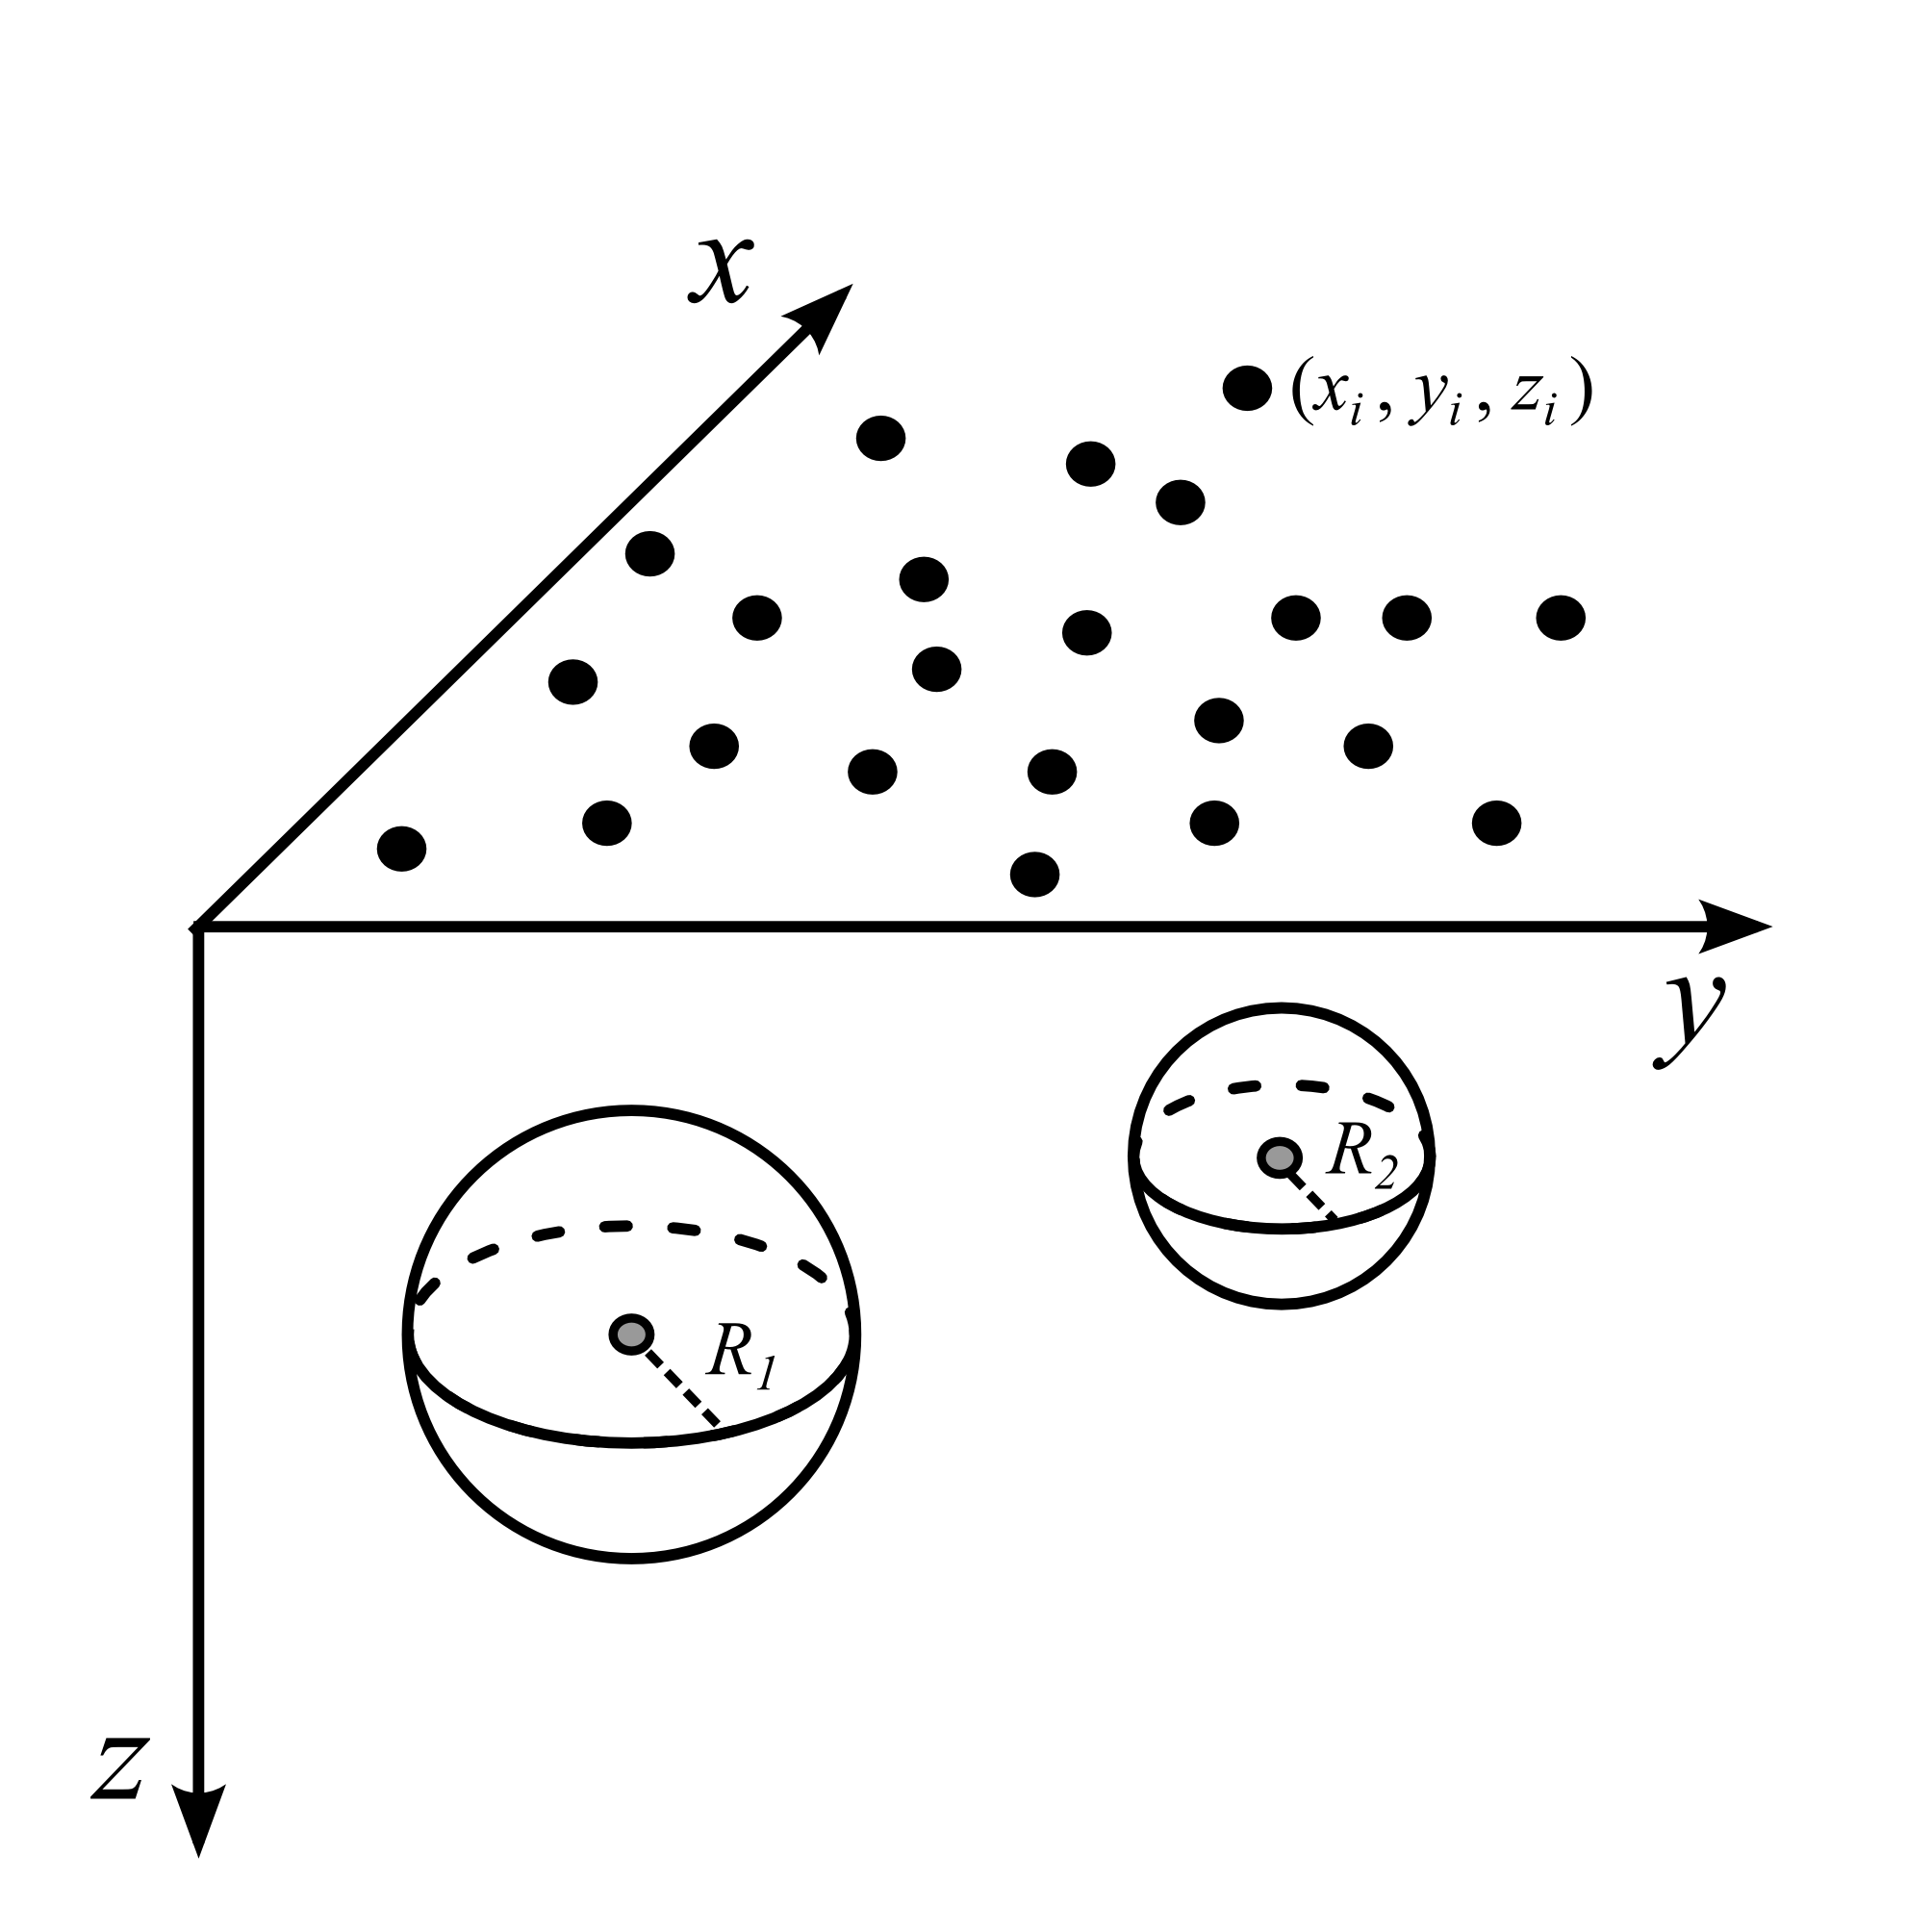
\includegraphics[width=90mm]{Figures/npgd-2014-0069-f01}
\caption{Schematic representation of $L = 2$ spheres uniformly
  magnetized at the subsurface. These spheres have radii $R_{j}$
  (dashed straight lines), constant magnetization vectors
  $\vec{m}^{j}$ and centres (grey dots) at ($xc_{j}$, $yc_{j}$, $zc_{j}$),
  $j = 1, \ldots, L$. The magnetic effect produced by these spheres
  can be observed at the points ($x_{i}$, $y_{i}$, $z_{i}$), $i = 1,
  \ldots, N$ (black dots). In this Cartesian coordinate system, $x$
  points to the geographic North, $y$ points to East and $z$ points
  downward.}
\label{fig:geometric-aspects}
\end{figure}

\begin{figure}[t]
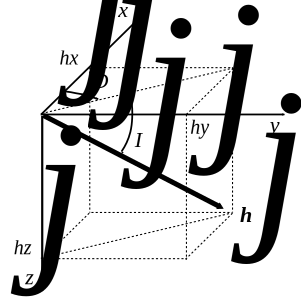
\includegraphics[width=80mm]{Figures/npgd-2014-0069-f02}
\caption{Schematic representation of the vector $\vec{h}^{j}$
  (Eq.~\ref{eq:hj}) with elements $hx_{j}$, $hy_{j}$ and $hz_{j}$ in
  Cartesian coordinates. This vector has a~declination $D_{j}$
  (positive in the clockwise sense) and inclination $I_{j}$ (positive
  downward), $j = 1, \ldots, L$.}
\label{fig:spherical-coordinates}
\end{figure}

\begin{figure}[t]
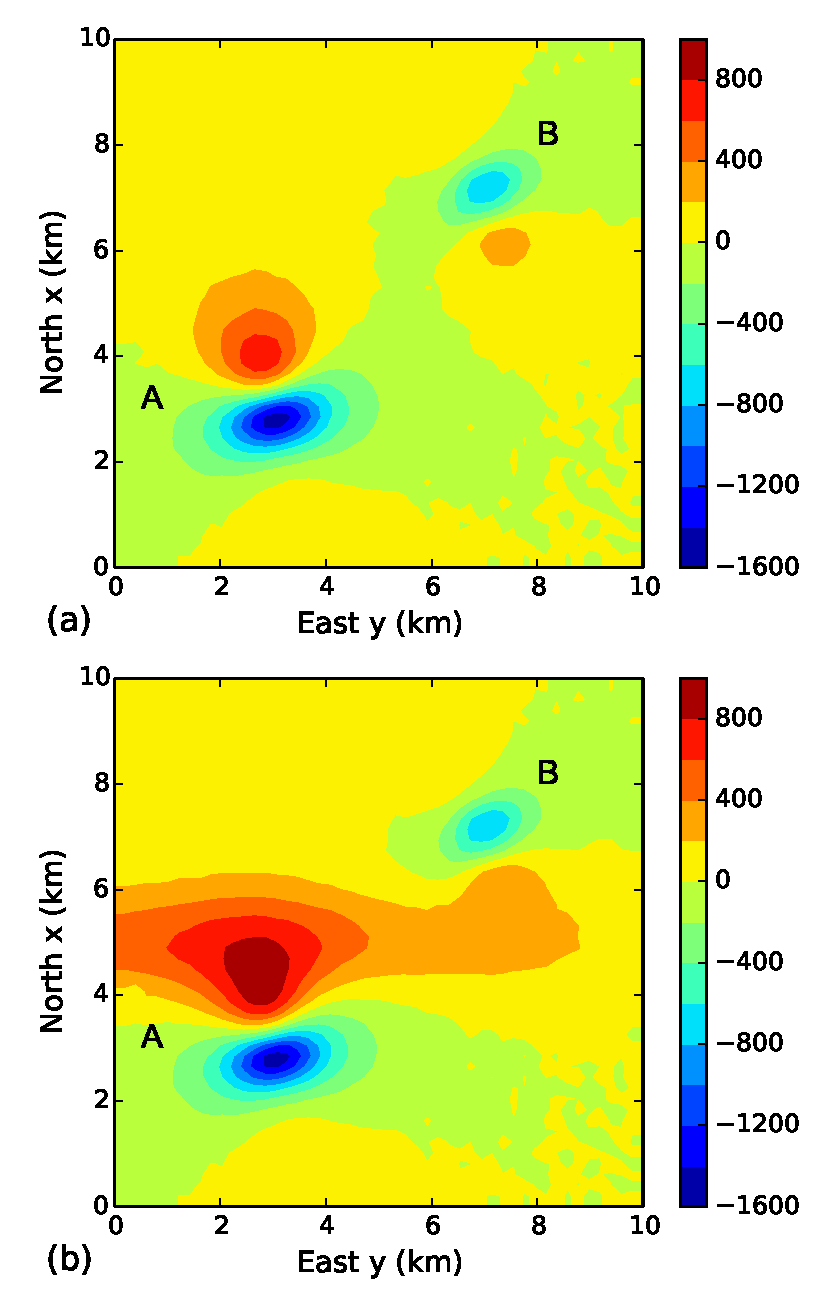
\includegraphics[width=50mm]{Figures/npgd-2014-0069-f03}
\caption{Validation test and robustness against interfering
  anomalies. \textbf{(a)} Synthetic noise-corrupted total field
  anomaly produced (nT) by a~sphere and a~rectangular
  prism. \textbf{(b)} Synthetic anomaly shown in \textbf{(a)} plus
  produced by an interfering anomaly. The anomalies produced by the
  sphere and prism are pinpointed as (A)~and (B),
  respectively.}
\label{fig:synt1-data}
\end{figure}

\begin{figure}[t]
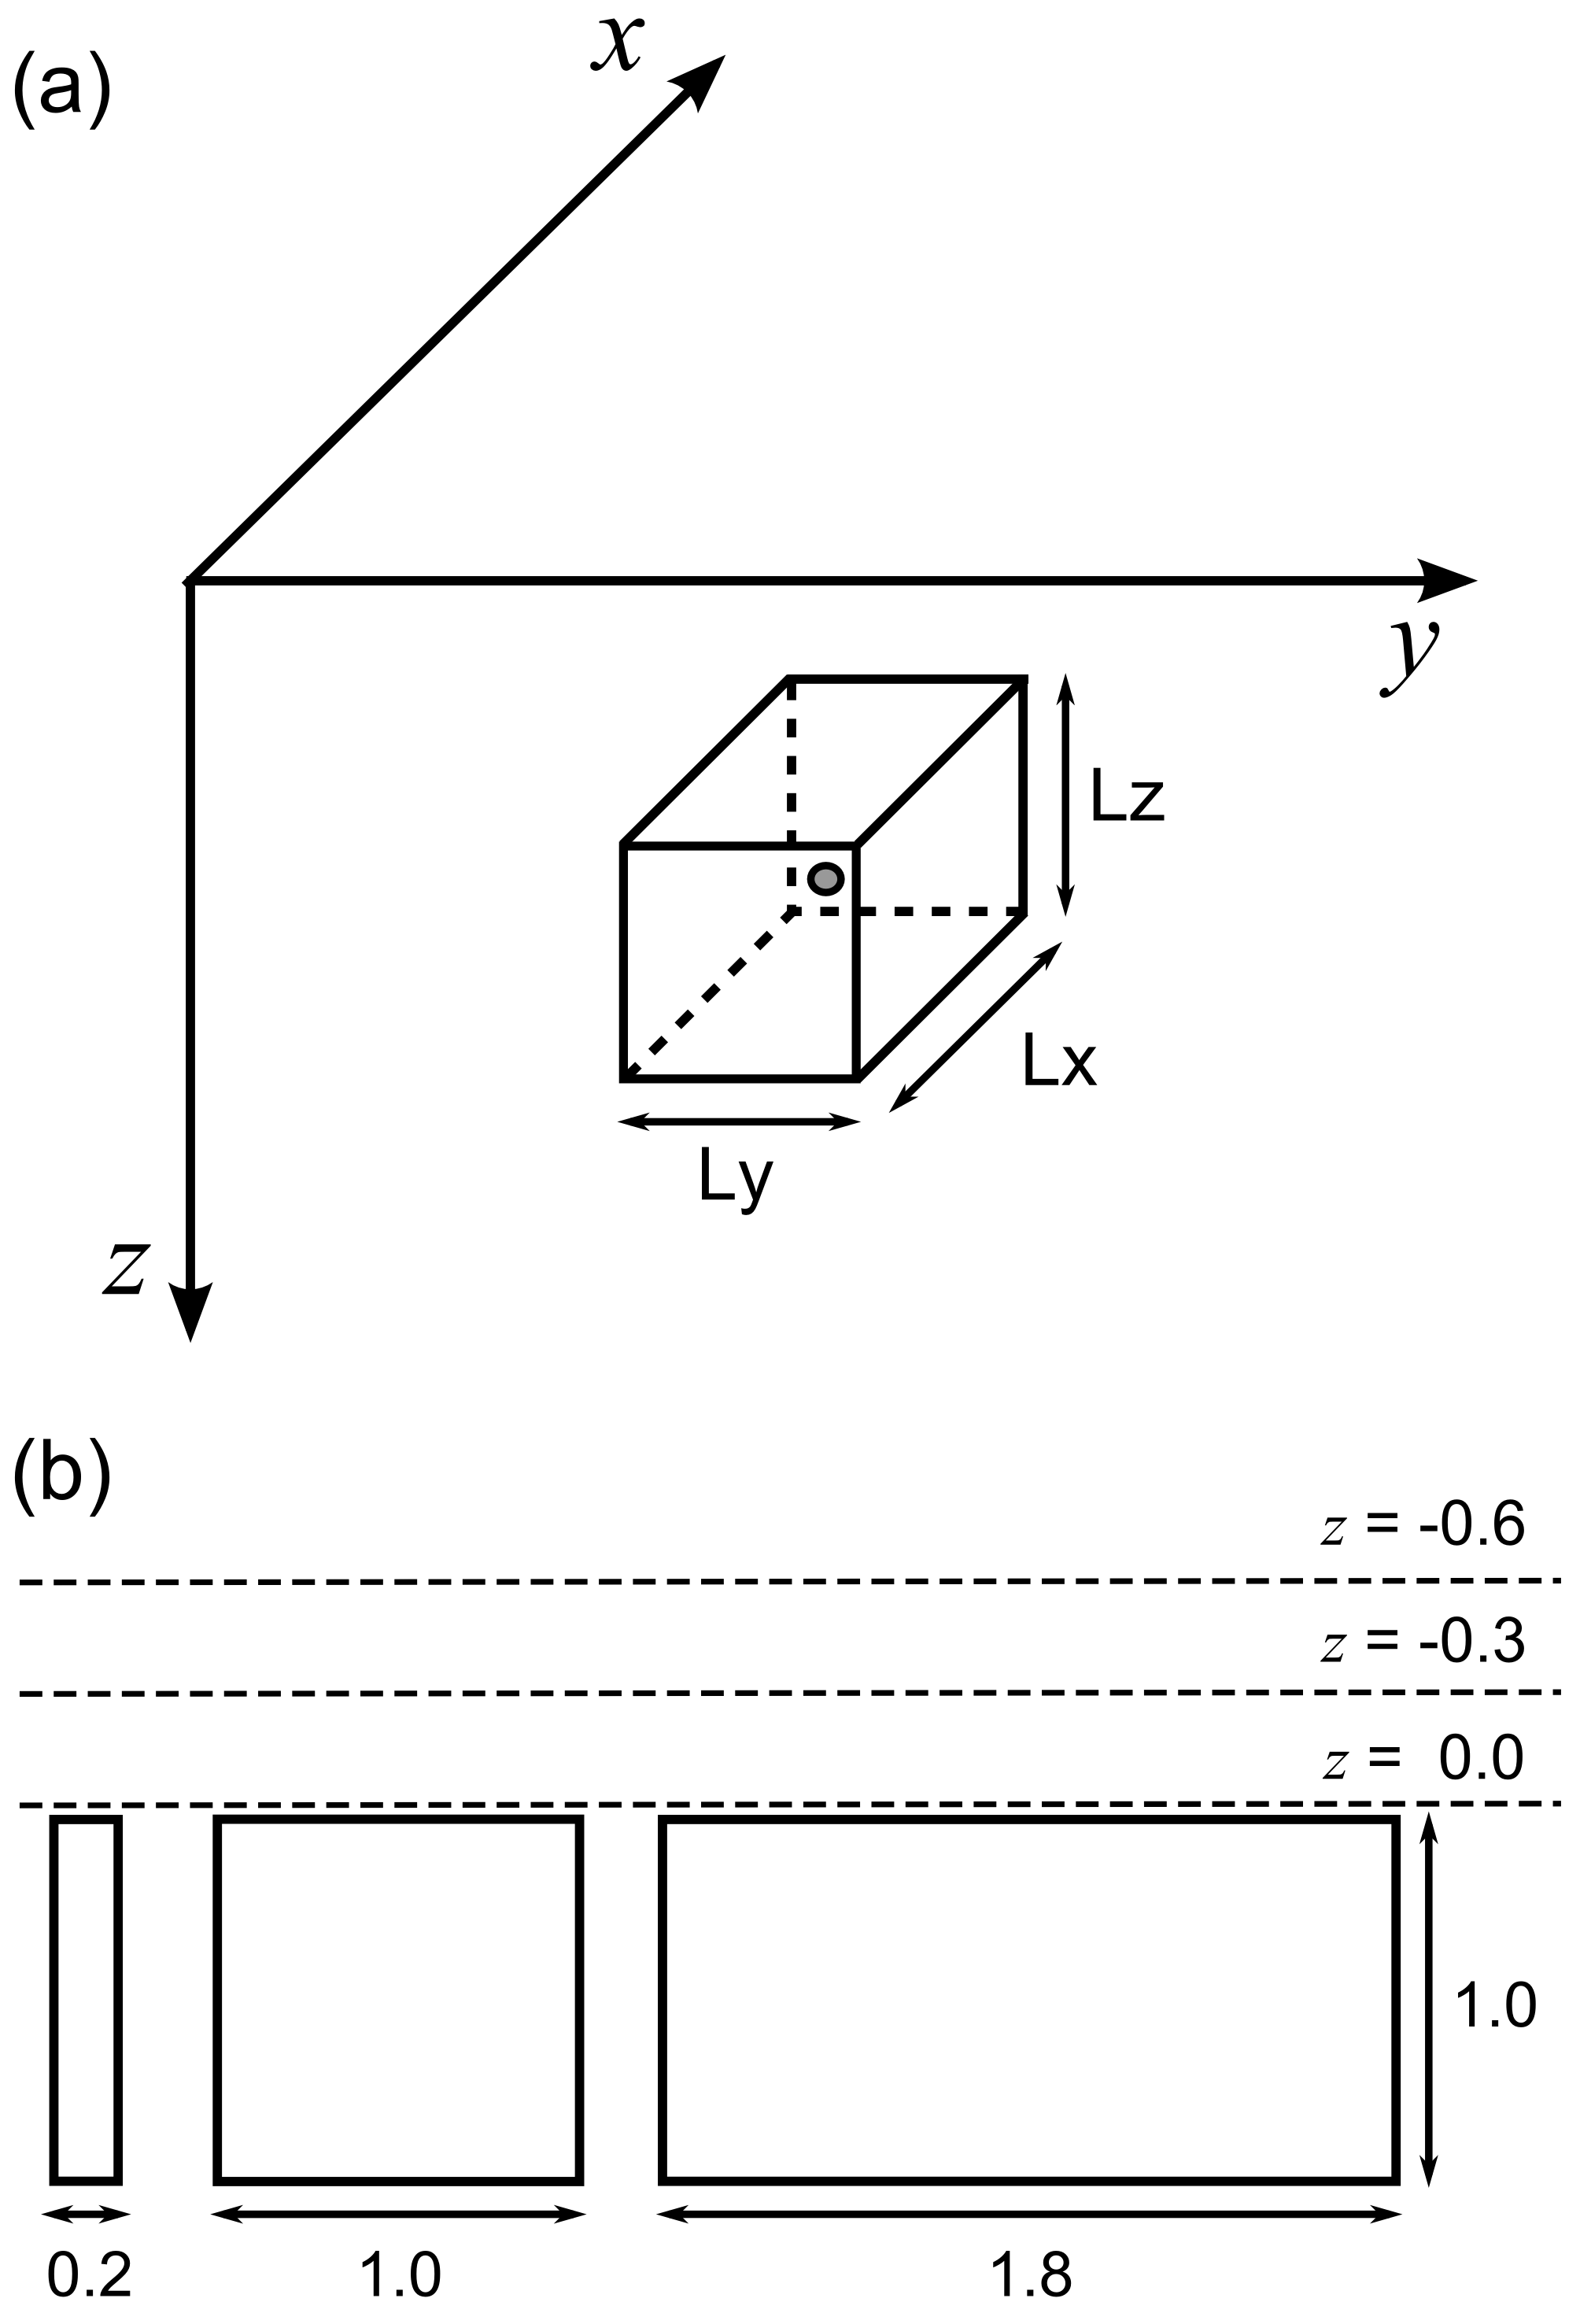
\includegraphics[width=68mm]{Figures/npgd-2014-0069-f04}
\caption{Robustness against non-spherical sources. \textbf{(a)} Rectangular
  prism with dimensions $Lx$, $Ly$ and $Lz$ and centre at the grey dot. \textbf{(b)}
  Projection of three prisms on the plane $yz$. All prisms have top at
  $z=10$\,\unit{m} and side lengths $Lx=Lz=1000$\,\unit{m}. The
  horizontal dimension $Ly$ of each prism is equal to $200$\,\unit{m},
  $1000$\,\unit{m} and $1800$\,\unit{m}. The dashed lines represent
  the vertical coordinate $z$ of three different horizontal planes
  above the prisms. For convenience, all coordinates and lengths are
  normalized by the numerical value of $Lz$ ($1000$\,\unit{m}) to
  obtain dimensionless quantities.}
\label{fig:robust-shape-methodology}
\end{figure}



\begin{figure*}[t]
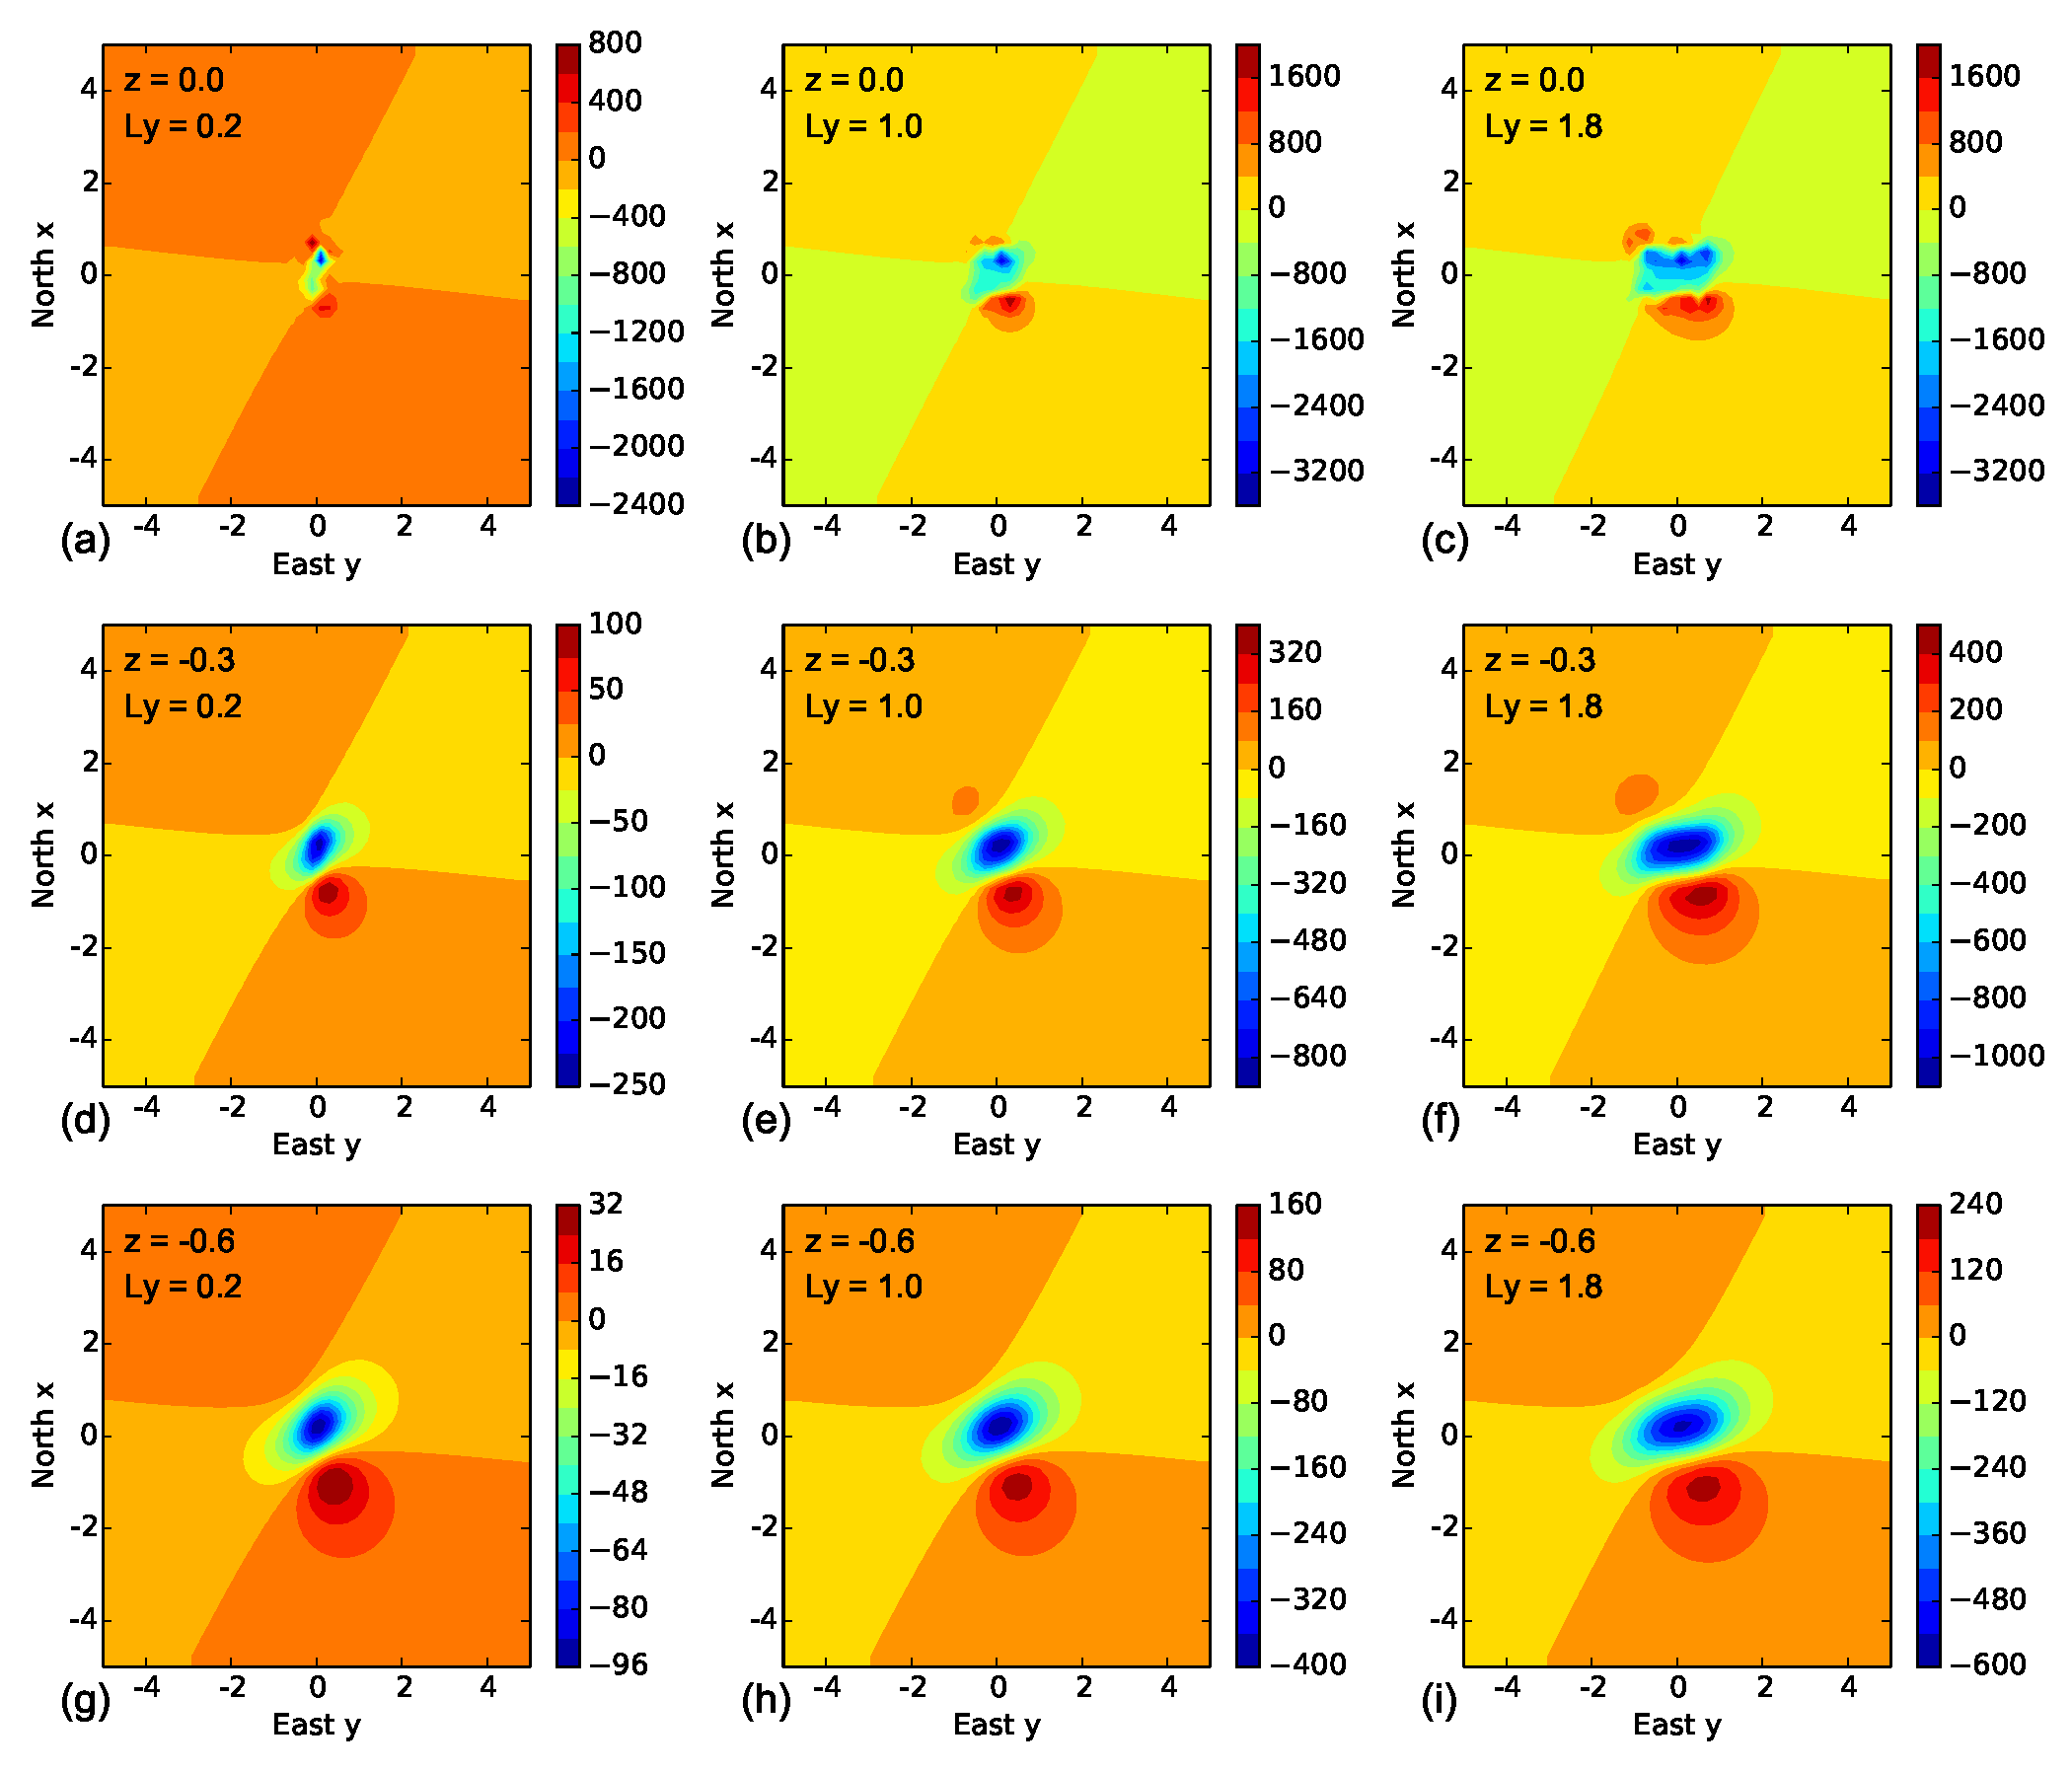
\includegraphics[width=110mm]{Figures/npgd-2014-0069-f05}
\caption{Robustness against non-spherical sources. Noise-corrupted
  total-field anomaly produced by each one of the three rectangular
  prisms shown in Fig.~\ref{fig:robust-shape-methodology}b on three
  horizontal planes with different constant vertical coordinates $z$
  (dashed lines in Fig.~\ref{fig:robust-shape-methodology}b). We
  consider that the centre of all prisms are located at $xc = 0.00$,
  $yc = 0.00$ and $zc = 0.51$.The intensity, declination and
  inclination of the magnetization vector of all prisms are equal to
  $6$\,\unit{A\,m^{-1}}, $-40${\degree} and $30${\degree},
  respectively. The simulated geomagnetic field is constant, with
  declination $-15${\degree} and inclination $-10${\degree}. The data
  are in nT and all coordinates and lengths are dimensionless (see
  Fig.~\ref{fig:robust-shape-methodology}).}
\label{fig:robust-shape-data}
\end{figure*}


\begin{figure}[t]
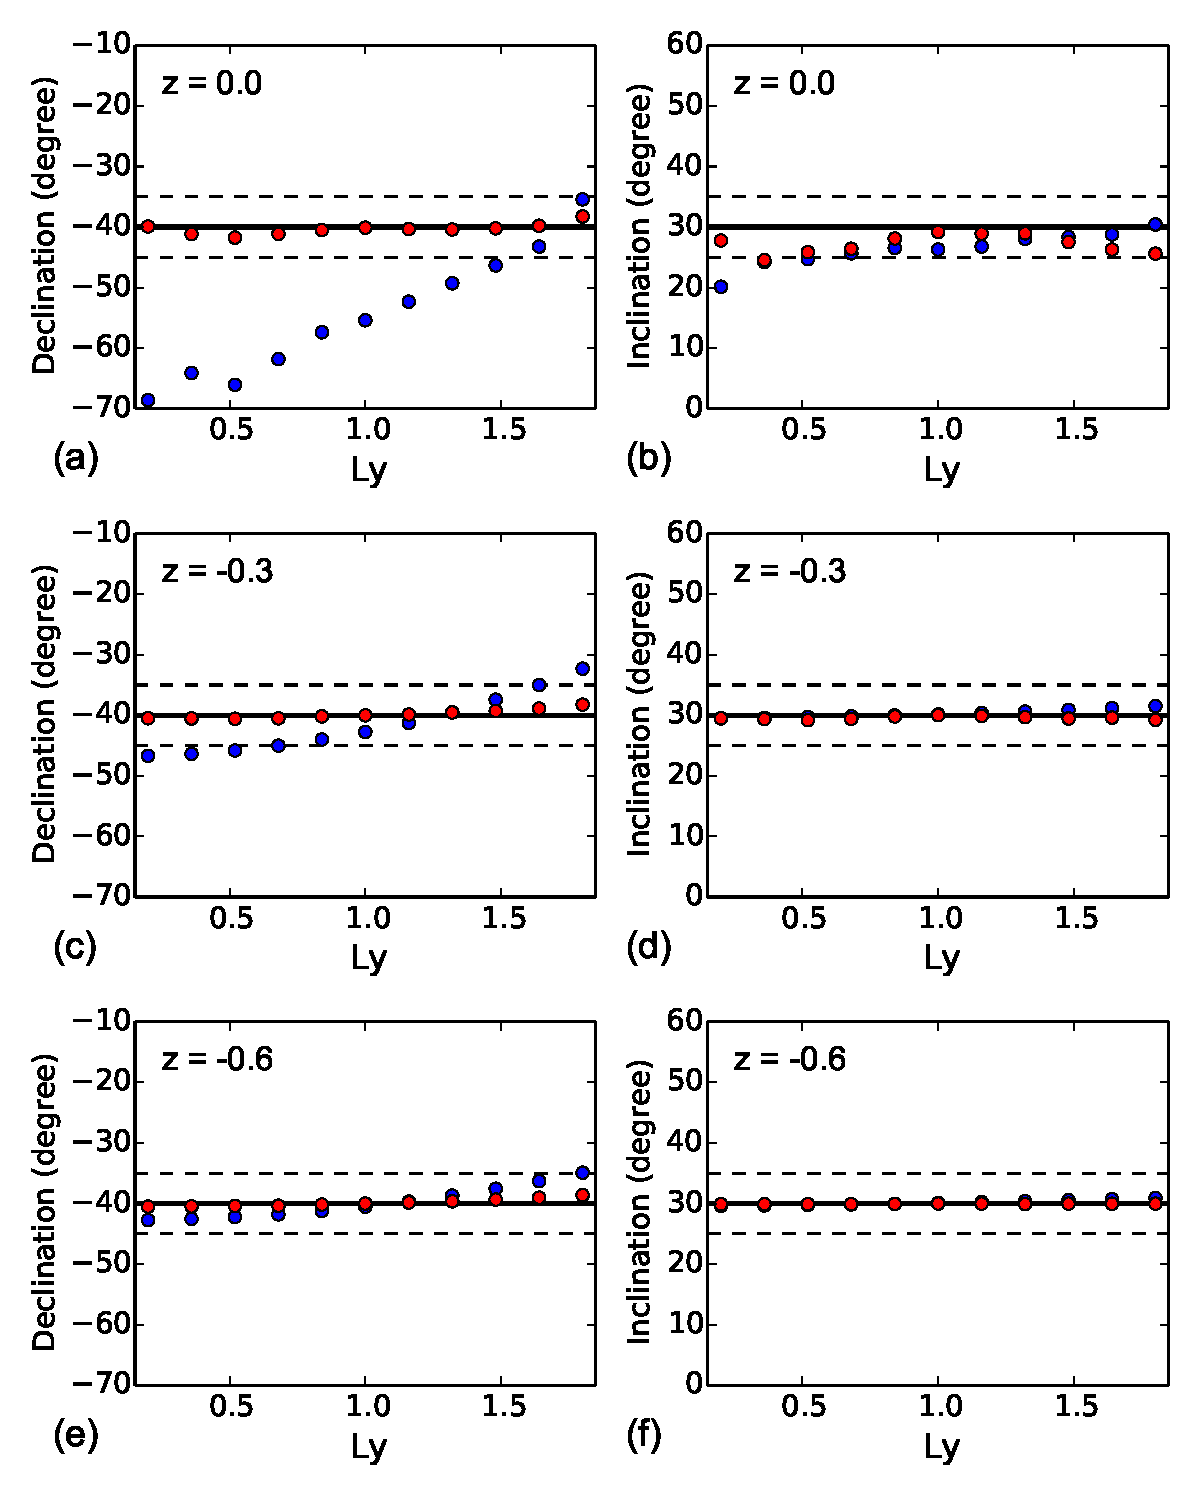
\includegraphics[width=80mm]{Figures/npgd-2014-0069-f06}
\caption{Robustness against non-spherical sources. The blue and red
  dots represent, respectively, the results obtained with the
  least-squares $\hat{\vec{h}}$ (Eq.~\ref{eq:h_hat}) and robust
  $\tilde{\vec{h}}$ (Eqs.~\ref{eq:iteration-L1} and \ref{eq:ri})
  estimates. Each dot represents an estimated declination or
  inclination obtained from the total-field anomaly produced by
  a~rectangular prism with a~different $Ly$
  (Fig.~\ref{fig:robust-shape-methodology}). $z$ indicates the constant
  vertical coordinate of the planar surface on which the total-field
  anomaly was calculated (dashed lines in
  Fig.~\ref{fig:robust-shape-methodology}b). The continuous black
  lines represent the true declinations (or inclinations). The dashed
  lines represent the true declination (or inclination) $\pm
  5${\degree}.}
\label{fig:robust-shape-results}
\end{figure}

\begin{figure}[t]
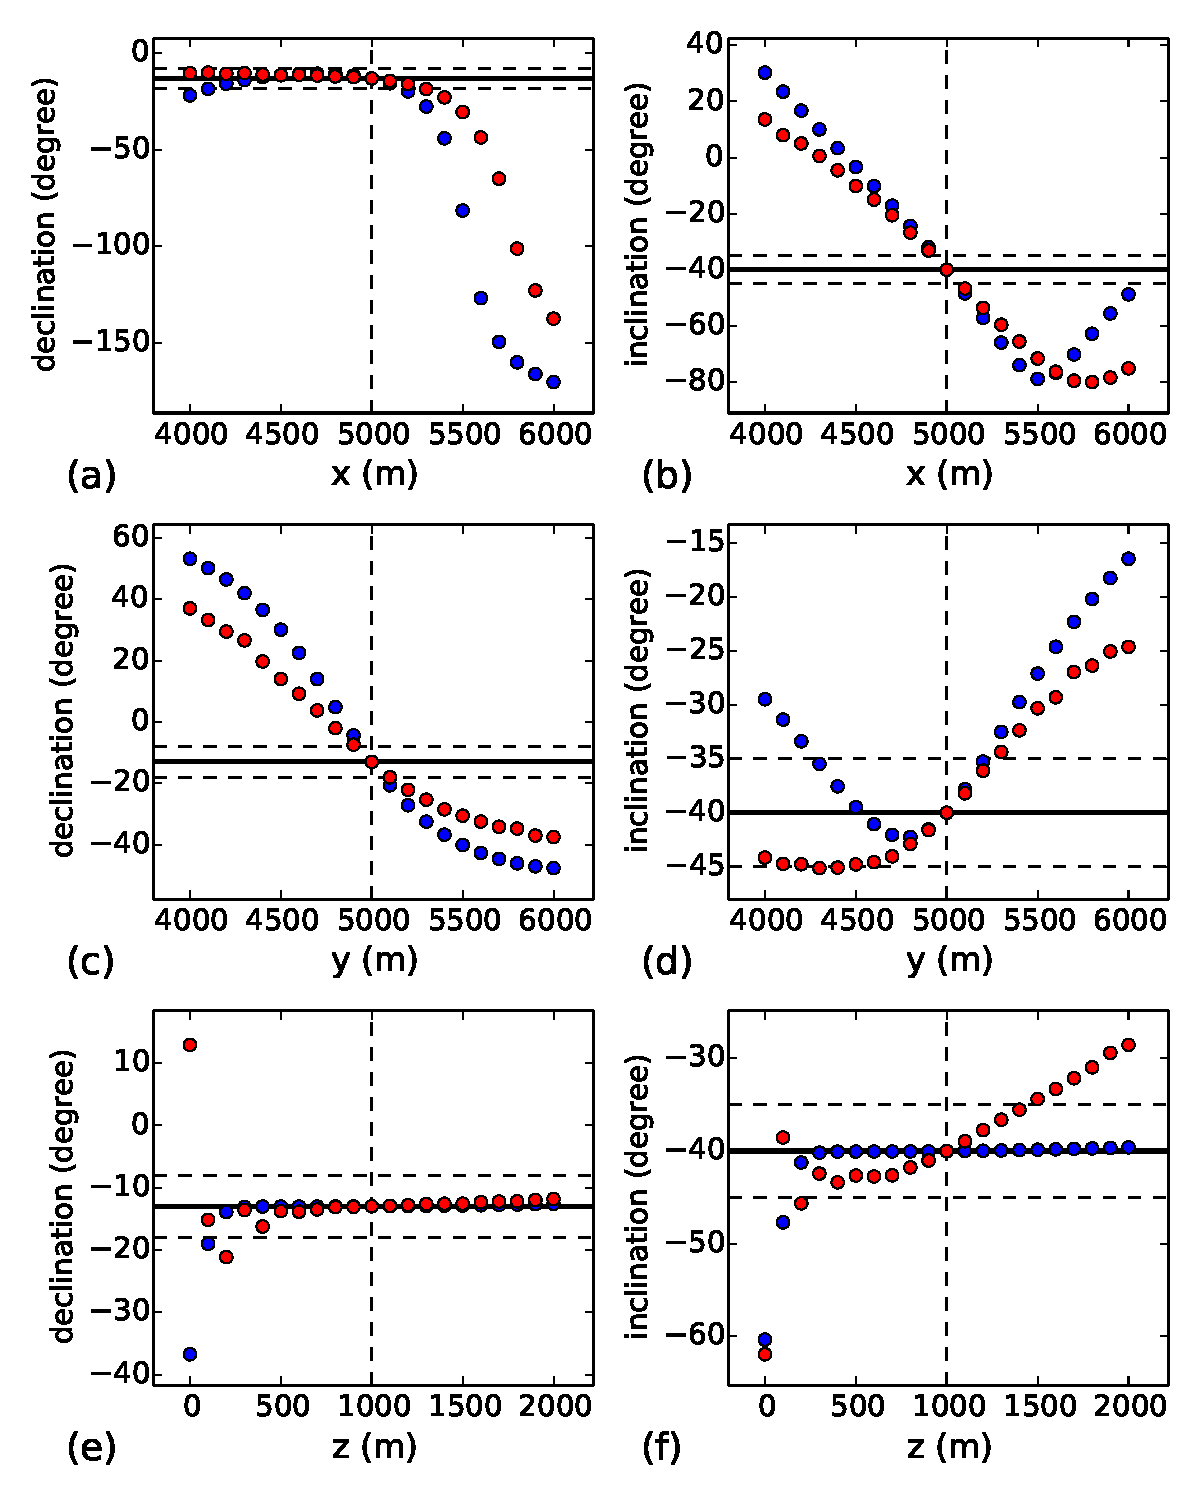
\includegraphics[width=70mm]{Figures/npgd-2014-0069-f07}
\caption{Robustness against errors in the centre location. The blue
  and red dots represent, respectively, the magnetization direction of
  a~simulated spherical body obtained with the least-squares
  $\hat{\vec{h}}$ (Eq.~\ref{eq:h_hat}) and robust $\tilde{\vec{h}}$
  (Eqs.~\ref{eq:iteration-L1} and \ref{eq:ri}) estimates. The
  estimated declinations and inclinations were obtained by presuming
    different positions for the centre of the source along the $x$, $y$ and
$z$~axis. Along each axis, the magnetization direction was
  estimated by considering $21$ different centres regularly spaced in
  a~range of 2000\,\unit{m} on a~line passing through the right
  coordinates of the centre of the simulated spherical body (vertical
  dashed lines). The continuous black lines represent the true
  declinations (or inclinations). The dashed lines represent the true
  declination (or inclination) $\pm 5${\degree}.}
\label{fig:robust-center-results}
\end{figure}

%New figures ==>

\begin{figure*}[t]
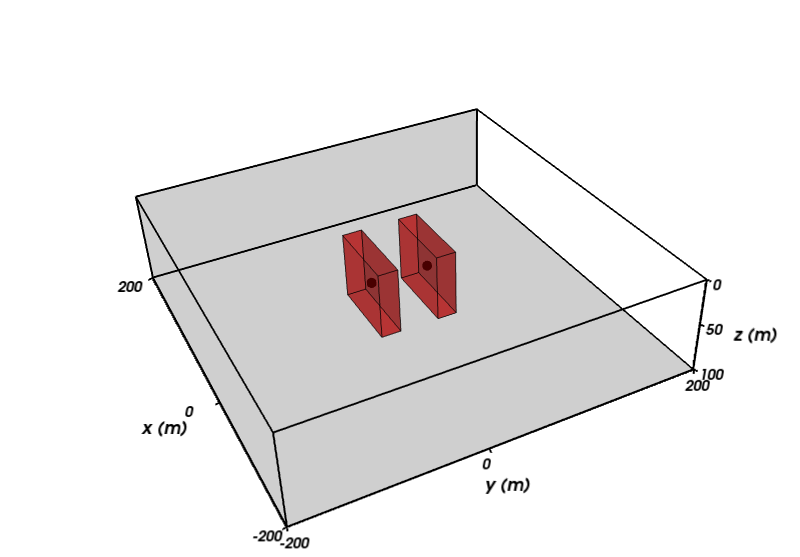
\includegraphics[width=120mm]{Figures/npgd-2014-0069-f08}
\caption{Strong-interfering anomalies. Synthetic prisms
(in red) with side lengths
equal to 80\,\unit{m}, 20\,\unit{m} and 70\,\unit{m} along
the $x$, $y$ and $z$ directions, respectively. Both prisms have a depth
of the top at $z = 10$\,\unit{m}. The eastern prism has its centre at
$xc = 0$\,\unit{m}, $yc = -30$\,\unit{m} and $zc = 45$\,\unit{m} while
western prism has its centre shifted 60\,\unit{m} in the positive $y$
direction (pinpointed black dots).}
\label{fig:overlapping-prisms}
\end{figure*}


\begin{figure*}[t]
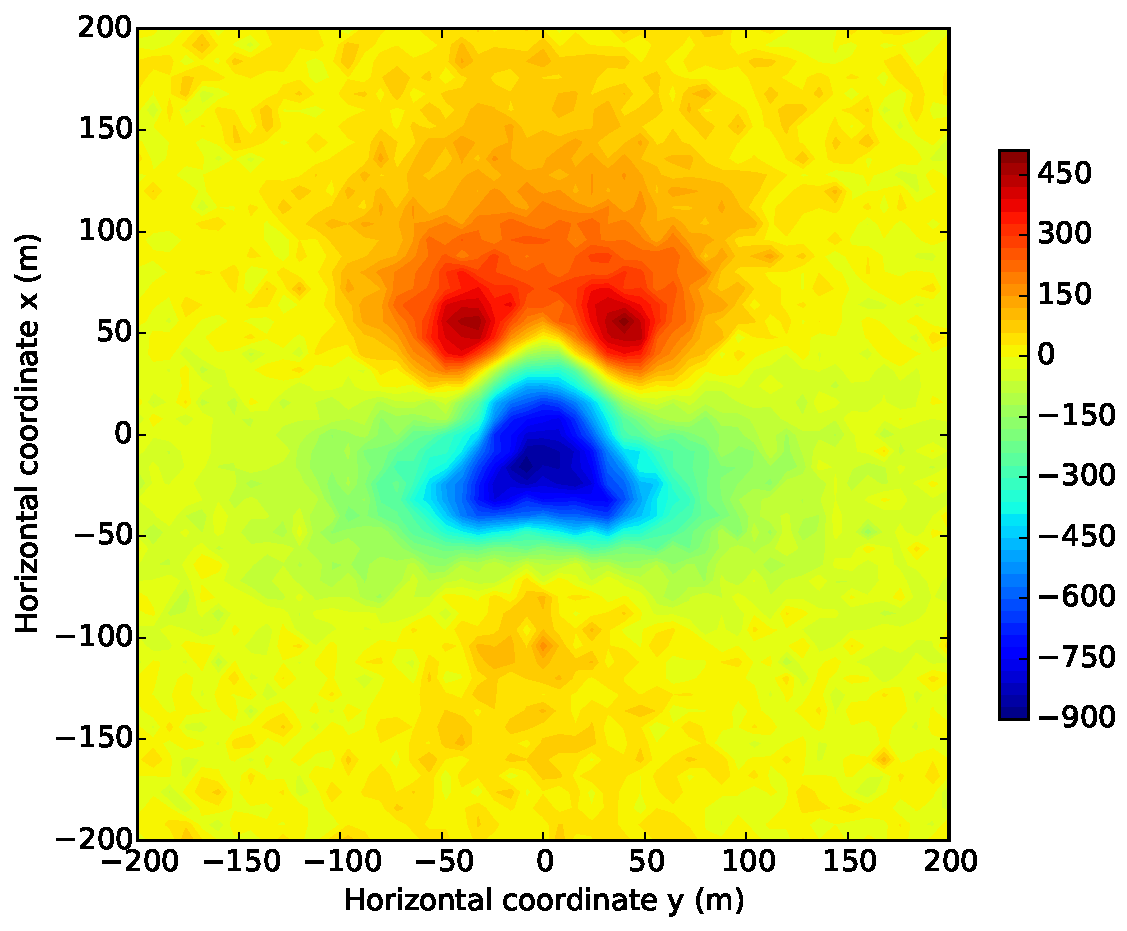
\includegraphics[width=120mm]{Figures/npgd-2014-0069-f09}
\caption{Strong-interfering anomalies. Noise-corrupted
total-field anomaly produced by the synthetic bodies shown in
Fig. \ref{fig:overlapping-prisms}. The data are in nT and were
calculated on a plane with constant vertical coordinate equal to
-10\,\unit{m}.}
\label{fig:overlapping-prisms-data}
\end{figure*}


\begin{figure*}[t]
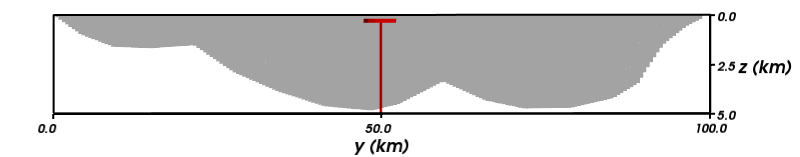
\includegraphics[width=120mm]{Figures/npgd-2014-0069-f10}
\caption{Igneous intrusion. 2D schematic representation of a
synthetic geologic setting composed of a nonmagnetic sedimentary 
package (in grey), an igneous intrusion
(in red) and a basement (in white). The sedimentary 
package and basement are semi-infinite along the $x$ axis. 
The basement is magnetized by 
induction and the intrusion has a strong reversed magnetization. The
plot has vertical exaggeration.}
\label{fig:intrusion-profile}
\end{figure*}

\begin{figure*}[t]
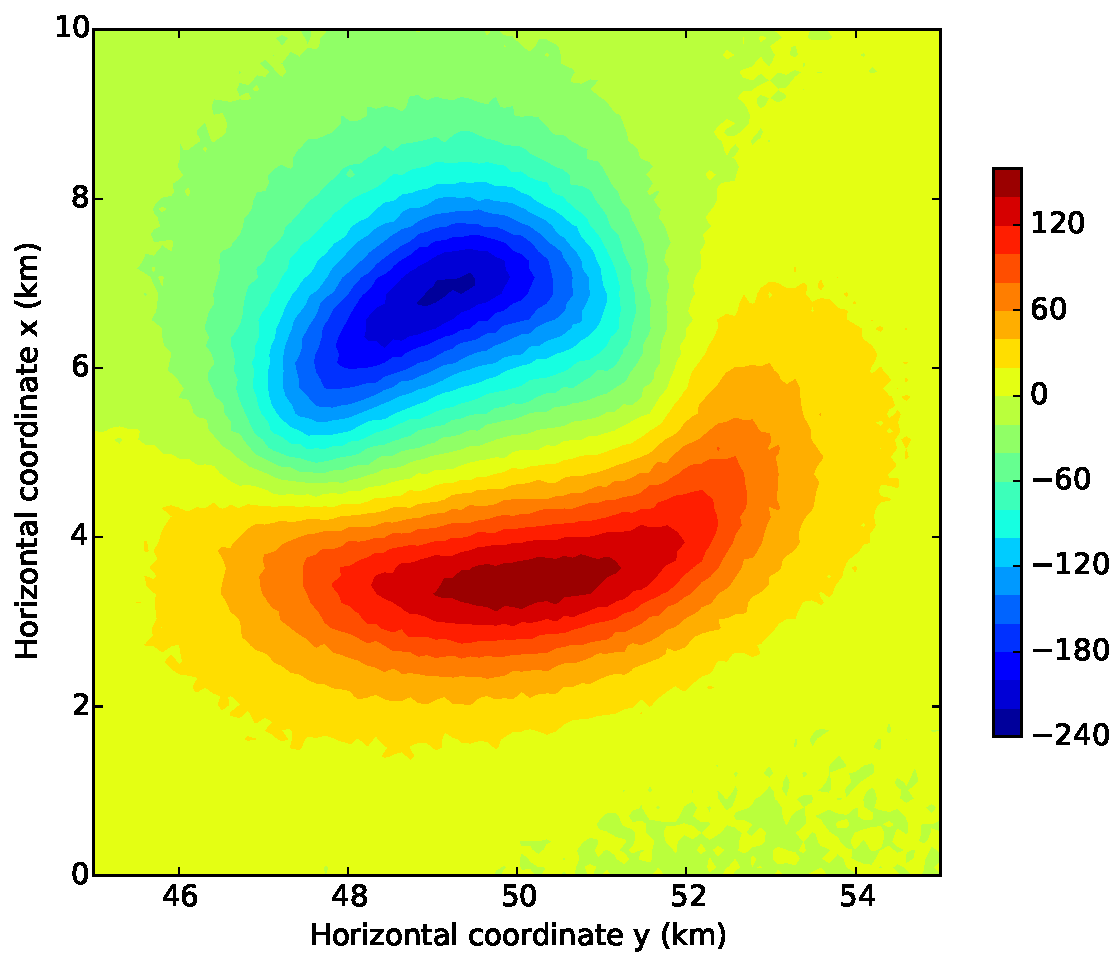
\includegraphics[width=120mm]{Figures/npgd-2014-0069-f11}
\caption{Igneous intrusion. Noise-corrupted total-field anomaly
produced by the synthetic bodies shown schematically in Fig. 
\ref{fig:intrusion-profile}. The data are in nT.}
\label{fig:intrusion-data}
\end{figure*}

\begin{figure*}[t]
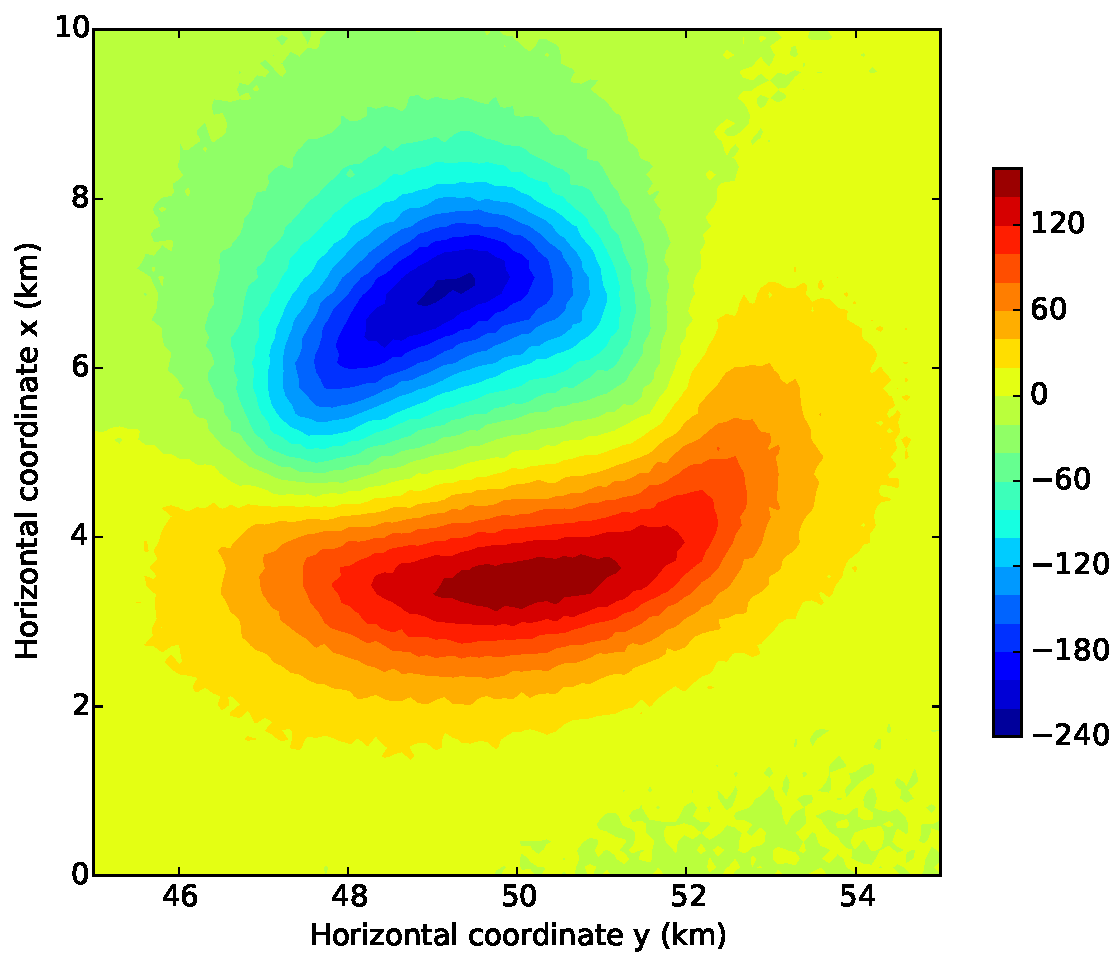
\includegraphics[width=120mm]{Figures/npgd-2014-0069-f12}
\caption{Igneous intrusion. 3D view of the intrusion (red prisms)
and the estimate of the intrusion position by
using Euler deconvolution (black point) with a structural 
index equal to 3. Notice
that the Euler solution falls outside the intrusion.}
\label{fig:intrusion-euler}
\end{figure*}

\begin{figure}[t]
  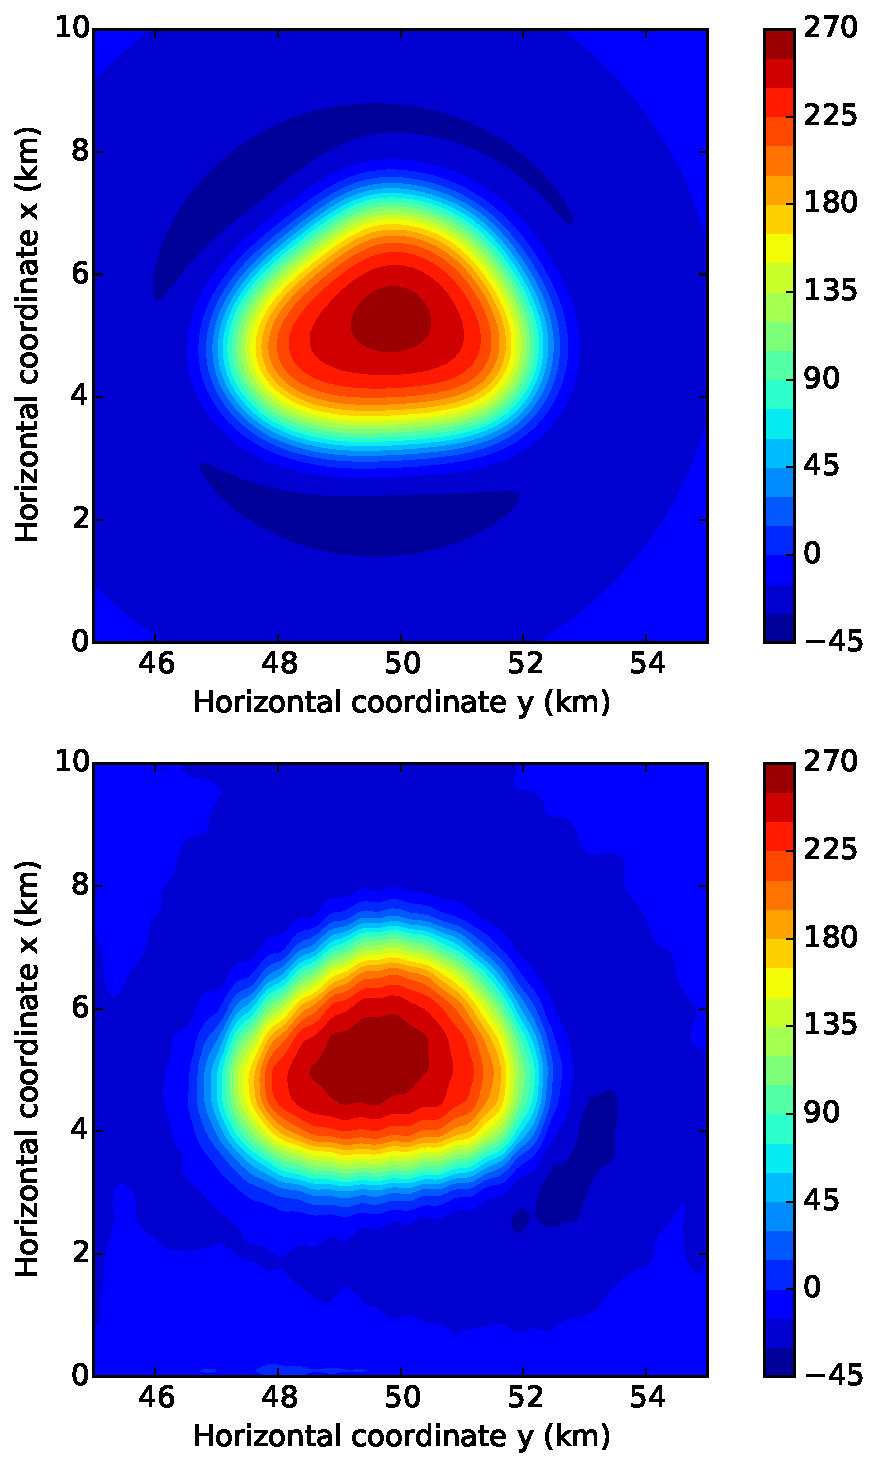
\includegraphics[width=70mm]{Figures/npgd-2014-0069-f13}
  \caption{Igneous intrusion. The upper panel shows the true
    reduced-to-the-pole anomaly produced by the synthetic bodies
    shown in Fig. \ref{fig:intrusion-profile}. The lower panel
    shows the reduced-to-the-pole anomaly obtained from the
    noise-corrupted total-field anomaly shown in Fig. \ref{fig:intrusion-data}.
    These anomalies were calculated at the same points of the
    total-field anomaly shown in Fig. \ref{fig:intrusion-data}.
    The reduction to the pole was calculated by using the robust estimates
    of declination $\tilde{D}$ and inclination $\tilde{I}$ shown
    in Tab. \ref{tab:intrusion-results}.}
\label{fig:intrusion-RTP}
\end{figure}

%<== New figures

\begin{figure*}[t]
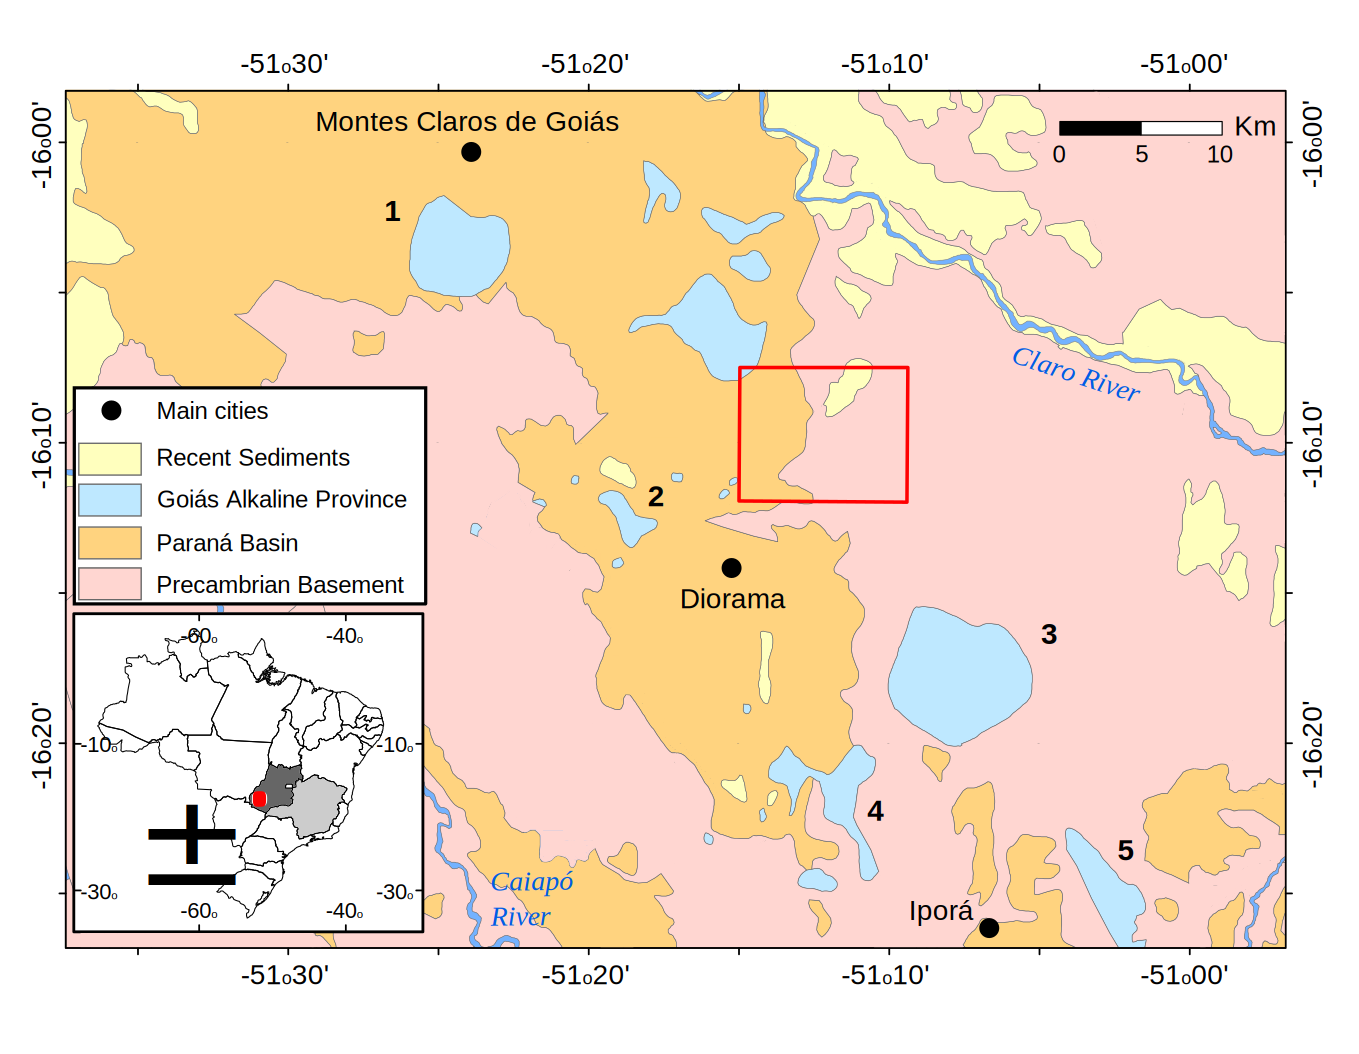
\includegraphics[width=120mm]{Figures/npgd-2014-0069-f14}
\caption{Application to field data on the Goi\'{a}s Alkaline Province
  (GAP), Brazil. Simplified geological map of the study area, which is
  shown as a~red dot in the inset map of Brazil. The inset also
  shows the Goi\'{a}s (dark grey area) and Minas Gerais (light grey
  area) states. The total-field anomaly over the area delimited by the
  red rectangle is shown in Fig.~\ref{fig:TFA-Diorama}. The
  coordinates are referred to the WGS84 datum. The numbers indicate
  the main alkaline complexes in this region: 1 -- Montes Claros de
  Goi\'{a}s, 2 -- Diorama, 3 -- C\'{o}rrego dos Bois, 4 -- Morro do
  Macaco and 5 -- Fazenda Buriti. }
\label{fig:geology-study-area}
\end{figure*}

\clearpage

\begin{figure*}[t]
  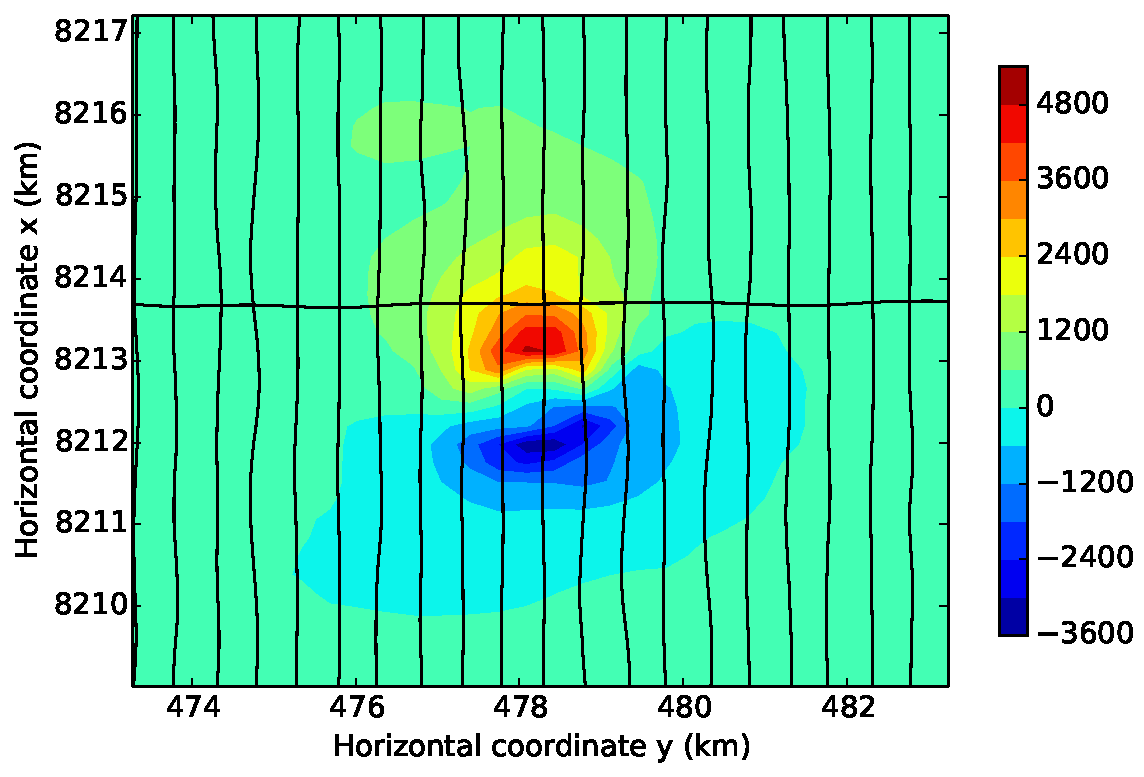
\includegraphics[width=120mm]{Figures/npgd-2014-0069-f15}
  \caption{Application to field data on the Goi\'{a}s Alkaline Province (GAP),
    Brazil. Total-field anomaly observed over the area delimited by the red
    rectangle in Fig.~\ref{fig:geology-study-area}. The flight lines of the
    aeromagnetic survey are shown in black. The magnetic data are in nT and the
    coordinates are in UTM on the SAD-69 datum, with central meridian
    $51${\degree}\,W. The origins of the east and north coordinates are 500 and
    10\,000\,\unit{km}, respectively.}
\label{fig:TFA-Diorama}
\end{figure*}

\clearpage

\begin{figure}[t]
  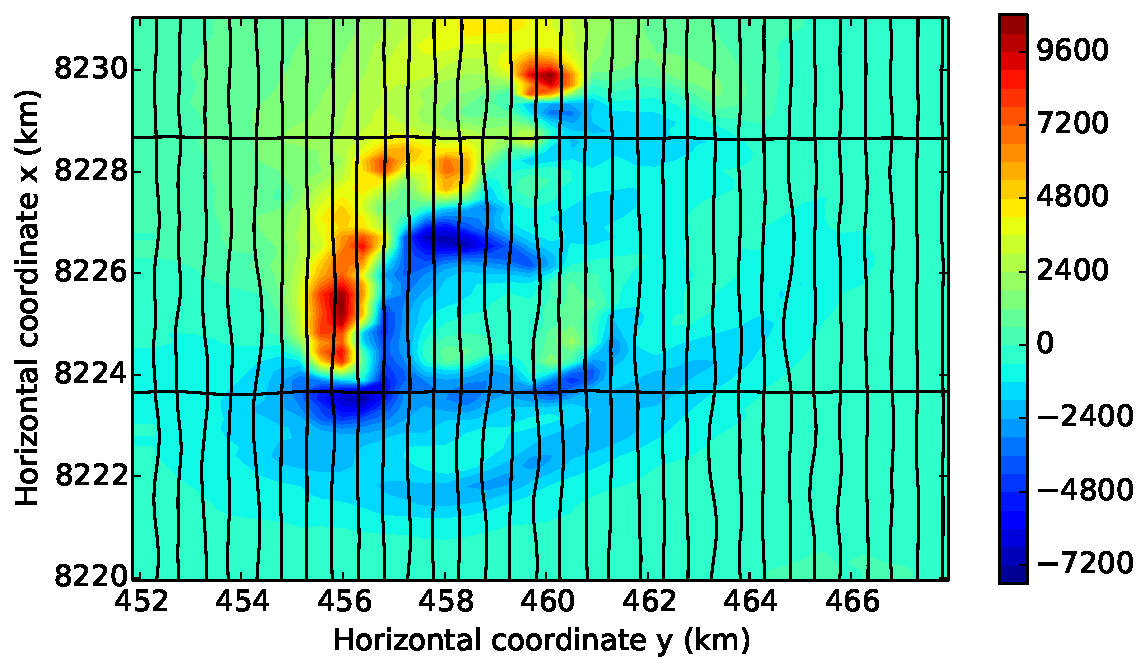
\includegraphics[width=70mm]{Figures/npgd-2014-0069-f16}
  \caption{Application to field data on the Goi\'{a}s Alkaline
    Province (GAP), Brazil. Observed total-field anomaly
    (Fig.~\ref{fig:TFA-Diorama}) reduced to the pole. The upper and
    lower panels show the RTP anomalies computed by using,
    respectively, the estimated magnetization direction obtained with
    the least-squares (inclination $\hat{I} = -69.25595{\degree} \pm
    0.00013${\degree} and declination $\hat{D} = -16.22821{\degree}
    \pm 0.00050${\degree}) and robust (inclination $\tilde{I} =
    -71.41751{\degree} \pm 0.00182${\degree} and declination
    $\tilde{D} = -23.39541{\degree} \pm 0.01049${\degree}) estimates. }
\label{fig:TFA-Diorama-RTP}
\end{figure}

\clearpage

\begin{figure*}[t]
  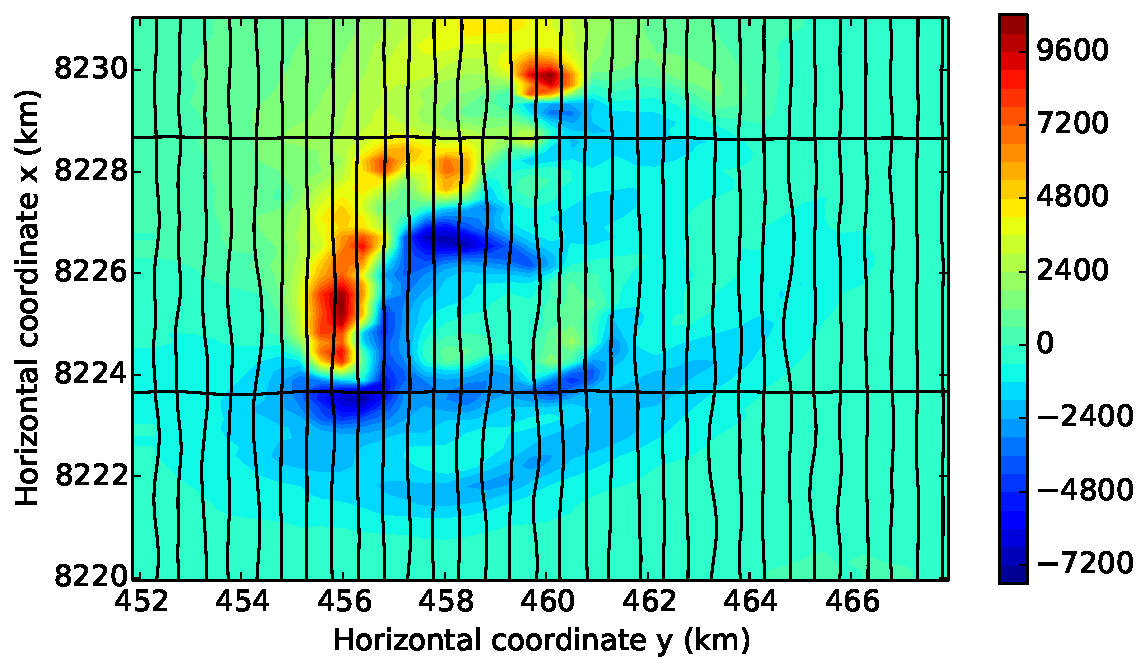
\includegraphics[width=120mm]{Figures/npgd-2014-0069-f17}
  \caption{Application to field data on the Goi\'{a}s Alkaline Province
    (GAP), Brazil. Total-field anomaly observed over the Montes Claros
    de Goi\'{a}s alkaline complex
    (Fig.~\ref{fig:geology-study-area}). The flight lines of the
    aeromagnetic survey are shown in black. The magnetic data are in nT
    and the coordinates are in UTM on the SAD-69 datum, with central
    meridian $51${\degree}\,W. The origins of the east and north
    coordinates are $500$\,\unit{km} and $10\,000$\,\unit{km},
    respectively. }
\label{fig:TFA-MCG}
\end{figure*}

\clearpage

\begin{figure}[t]
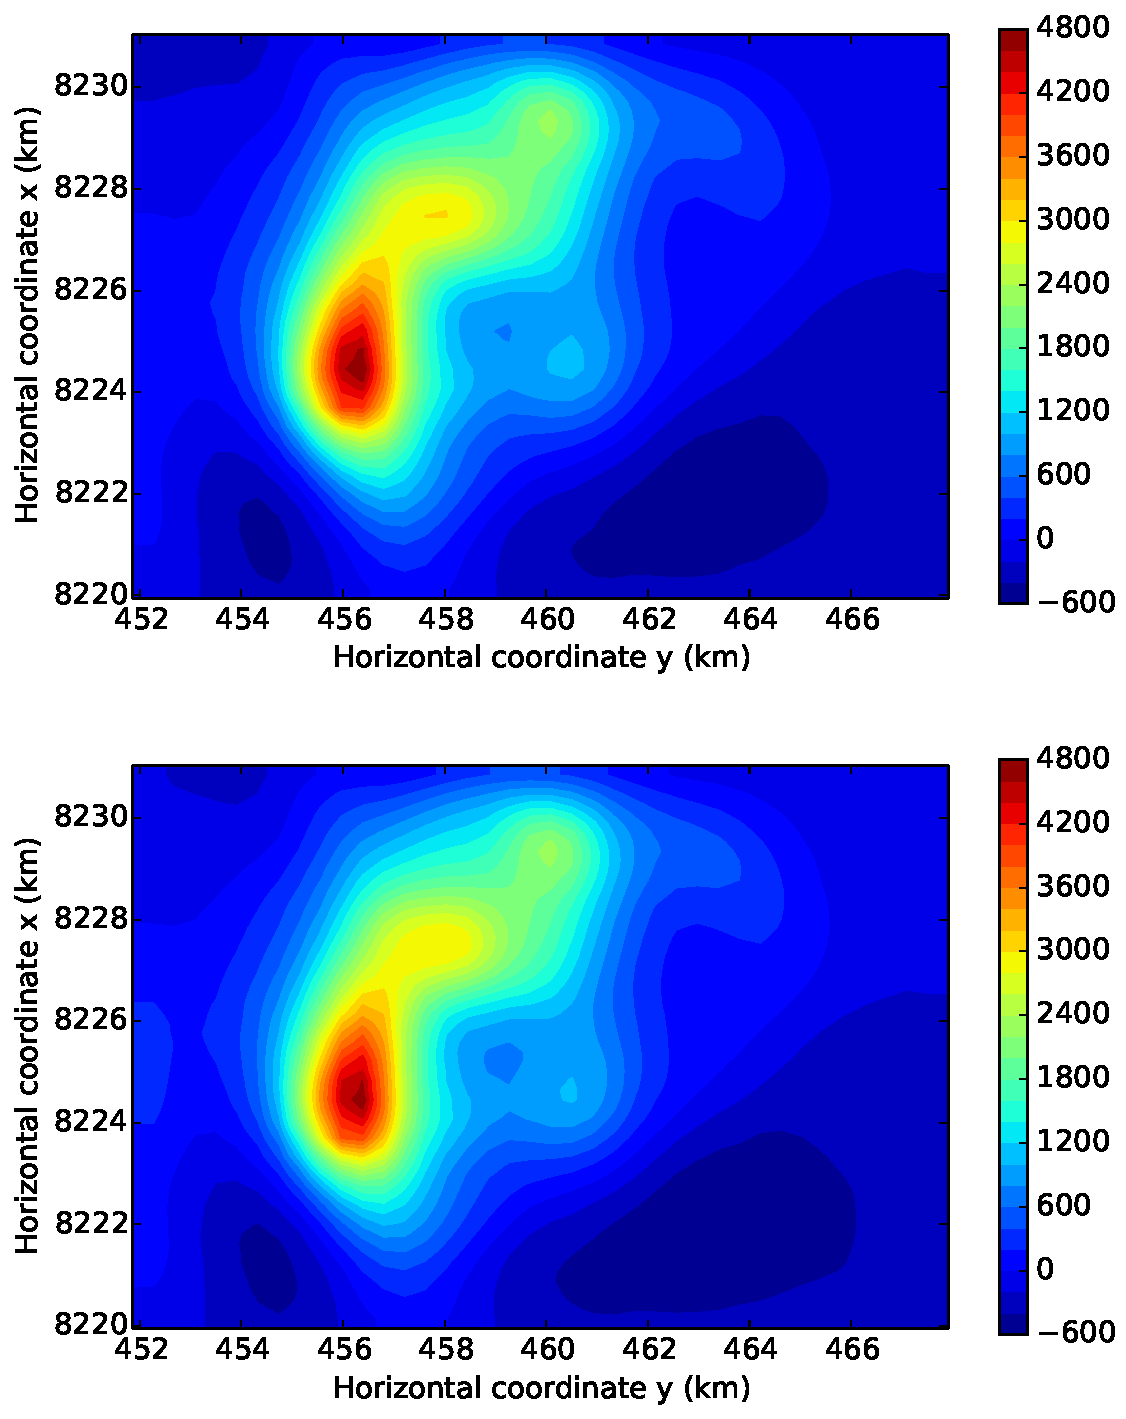
\includegraphics[width=80mm]{Figures/npgd-2014-0069-f18}
\caption{Application to field data on the Goi\'{a}s Alkaline Province
  (GAP), Brazil. Observed total-field anomaly (Fig.~\ref{fig:TFA-MCG})
  reduced to the pole. The upper and lower panels show the RTP
  anomalies computed by using, respectively, the estimated
  magnetization direction obtained with the least-squares (inclination
  $\hat{I} = -69.25595{\degree} \pm 0.00013${\degree} and declination
  $\hat{D} = -16.22821{\degree} \pm 0.00050${\degree}) and robust
  (inclination $\tilde{I} = -71.41751{\degree} \pm 0.00182${\degree}
  and declination $\tilde{D} = -23.39541{\degree} \pm
  0.01049${\degree}) estimates. }
\label{fig:TFA-MCG-RTP}
\end{figure}


\end{document}

